\documentclass[UTF8, 10pt, nonatbib, nocopyrightspace, reprint]{sigplanconf}

\usepackage[backref=section, linkbordercolor={1 1 1}, urlbordercolor={1 1 1}, citebordercolor={1 1 1}]{hyperref}
\usepackage[ruled, vlined]{algorithm2e}
\usepackage{placeins}
\usepackage{color}
\usepackage{cite}
\usepackage{float}
\usepackage{graphicx}
\usepackage{parskip}
\usepackage{bytefield}
\usepackage{booktabs}
\usepackage{float}
\usepackage{tabularx}
\usepackage{pgfplots}
\usepackage{amsmath}
\usepackage{titlesec}
\usepackage[printwatermark]{xwatermark}

\graphicspath{ {images/} }

\newcommand{\todo}[1]{}
\renewcommand{\todo}[1]{{\color{red} TODO:\ {#1}}}

\SetAlgorithmName{Protocol}{Protocol}{List of Protocols}

%% 'DRAFT' Watermark
\newsavebox\mybox
\savebox\mybox{\tikz[color=black,opacity=0.05]\node{DRAFT};}
\newwatermark*[
 allpages,
 angle=45,
 scale=10,
 xpos=0,
 ypos=0
]{\usebox\mybox}

% Define the protocol environment
\newenvironment{protocol}[2]{
  \begin{algorithm}[!htb]
    \DontPrintSemicolon
    \caption{#1}\label{#2}
}{
  \end{algorithm}
  \FloatBarrier
}

\newcommand{\protoref}[1]{[\autoref{#1}]}

\renewcommand{\sectionautorefname}{Section}
\renewcommand{\subsectionautorefname}{Section}
\renewcommand{\subsubsectionautorefname}{Section}
\newcommand{\secref}[1]{[\autoref{#1}]}

\renewcommand{\figureautorefname}{Figure}
\newcommand{\figref}[1]{[\autoref{#1}]}



\pgfplotsset{compat=1.14}

\begin{document}

\special{papersize=8.5in,11in}
\setlength{\pdfpageheight}{\paperheight}
\setlength{\pdfpagewidth}{\paperwidth}

\title{Helium}
\subtitle{A Decentralized Machine Network}
\authorinfo{Amir Haleem\and Andrew Allen \and Andrew Thompson \and Marc Nijdam \and Rahul Garg}{Helium Systems, Inc.}{\today}

\maketitle

\begin{abstract}
The Internet of Things is an \textdollar800 billion industry, with over 8.4 billion connected devices online, and spending predicted to reach nearly \textdollar1.4 trillion by 2021~\cite{idc}. Most of these devices need to connect to the internet to function. However, current solutions such as cellular, WiFi, and Bluetooth are suboptimal: they are too expensive, too power hungry, or too limited in range.

Helium is a \emph{decentralized machine network} that enables devices anywhere in the world to wirelessly connect to the internet and geolocate themselves without the need for power-hungry satellite location hardware or expensive cellular plans. Powering the network is a blockchain with a native protocol token incentivizing a two-sided marketplace between coverage providers and coverage consumers. With the introduction of a blockchain, Helium injects decentralization into an industry currently controlled by monopolies. The result is that wireless network coverage becomes a commodity, fueled by competition, available anywhere in the world, at a fraction of current costs.

Helium's secure and open-source primitives enable developers to build low-power, internet-connected devices quickly and cost-effectively. Helium has a wide variety of applications across industries and is the first decentralized machine network of its kind.
\end{abstract}

%\newpage

%\tableofcontents
%\newpage

\section{Introduction}

The world is becoming decentralized. A multitude of platforms, technologies, and services are moving from centralized proprietary systems to decentralized, open ones. Peer-to-peer networks such as Napster (created by Helium founder Shawn Fanning) \cite{napster} and BitTorrent paved the way for blockchain networks and crypto-currencies to be built. Now Bitcoin, Ethereum, and other blockchain networks have shown the value of decentralized transaction ledgers. Existing internet services such as file storage, identity verification, and the domain name system are being replaced by modern blockchain-based versions. While software-level decentralization has moved quickly, physical networks are taking longer to affect. These networks are more complicated to decentralize as they often require specialized hardware to function.

Helium is a wide-area wireless networking system, a blockchain, and a protocol token. The blockchain runs on a new kind of proof, called \emph{Proof-of-Coverage}, where blocks are created by miners who are providing wireless network coverage in a cryptographically verified physical location and time. The Helium protocol provides a bi-directional data transfer system between wireless devices and the Internet via a network of independent providers that does not rely on a single coordinator, where: (1) devices pay to send \& receive data to the internet and geolocate themselves, (2) miners earn tokens for providing network coverage, and (3) miners earn fees from transactions, and for validating the integrity of the network.

\subsection{Key Components}

Helium is built around the following key components:

\begin{enumerate}
  \item \textbf{\emph{Proof-of-Coverage}}: we present a computationally-inexpensive \emph{Proof-of-Coverage} that allows miners to prove they are capable of providing wireless network coverage. We anchor these proofs using a \emph{Proof-of-Serialization} that allows miners to prove they are accurately representing time relative to others on the network in a cryptographically secure way.

  \item \textbf{Blockchain Network}: we demonstrate an entirely new purpose-built blockchain network built to service the \emph{Wireless Protocol} and provide a system for authenticating and identifying devices, providing cryptographic guarantees of data transmission and authenticity, offer transaction primitives designed around the wireless protocol, and more.

  \item \textbf{Helium Consensus Protocol}: we present a novel consensus protocol construction that creates a permisionless, high throughput, censor-resistant system by combining an asynchronous Byzantine Fault Tolerant protocol with identities presented via \emph{Proof-of-Coverage}. 

  \item \textbf{Wireless Protocol}: we introduce a new open-source and standards-compliant wireless network protocol, called \emph{WHIP}, designed for low power devices over vast areas. This protocol is designed to run on existing commodity radio chips available from dozens of manufacturers with no proprietary technologies or modulation schemes required.

  \item \textbf{\emph{Proof-of-Location}}: we outline a system for interpreting the physical \emph{geolocation} of a device using WHIP without the need for expensive and power-hungry satellite location hardware. Devices can make immutable, secure, and verifiable claims about their location at a given moment in time which is recorded in the blockchain.
\end{enumerate}

\subsection{System Overview}

\begin{itemize}
    \item Helium is a \emph{Decentralized Machine Network} built around a new wireless protocol (WHIP) on a purpose-built blockchain with a native token.
    \item Devices take the form of hardware containing a radio chip and firmware compatible with WHIP, and spend tokens by paying miners to send data to and from the internet.
    \item Miners earn tokens by providing wireless network coverage via purpose-built hardware which provides a bridge between WHIP and routers, which are internet applications.
    \item Devices store their private keys in commodity key-storage hardware and their public keys in the blockchain.
    \item Miners join the network by asserting their satellite-derived location, a special type of transaction in the blockchain, and staking a token deposit.
    \item Miners specify the price they are willing to accept for data transport and \emph{Proof-of-Location}, and devices specify the price they are willing to pay. Miners are paid once they prove they have delivered data to the devices' specified internet endpoint.
    \item Miners participate in the creation of new blocks in the blockchain by being elected to an asynchronous Byzantine Fault Tolerant consensus group.
    \item Miners are rewarded with newly minted Helium for blocks that are created while they are part of the consensus group. 
    \item A miner's probability of being elected to the consensus group at a given epoch is based on the quality of the wireless network coverage they provide.
    \item The blockchain employs \emph{Proof-of-Coverage} to guarantee that miners are honestly representing the wireless network coverage they are creating.
\end{itemize}

\figref{fig:system} shows a visual representation of the Helium network.

\begin{figure*}[ht]
    \begin{center}
          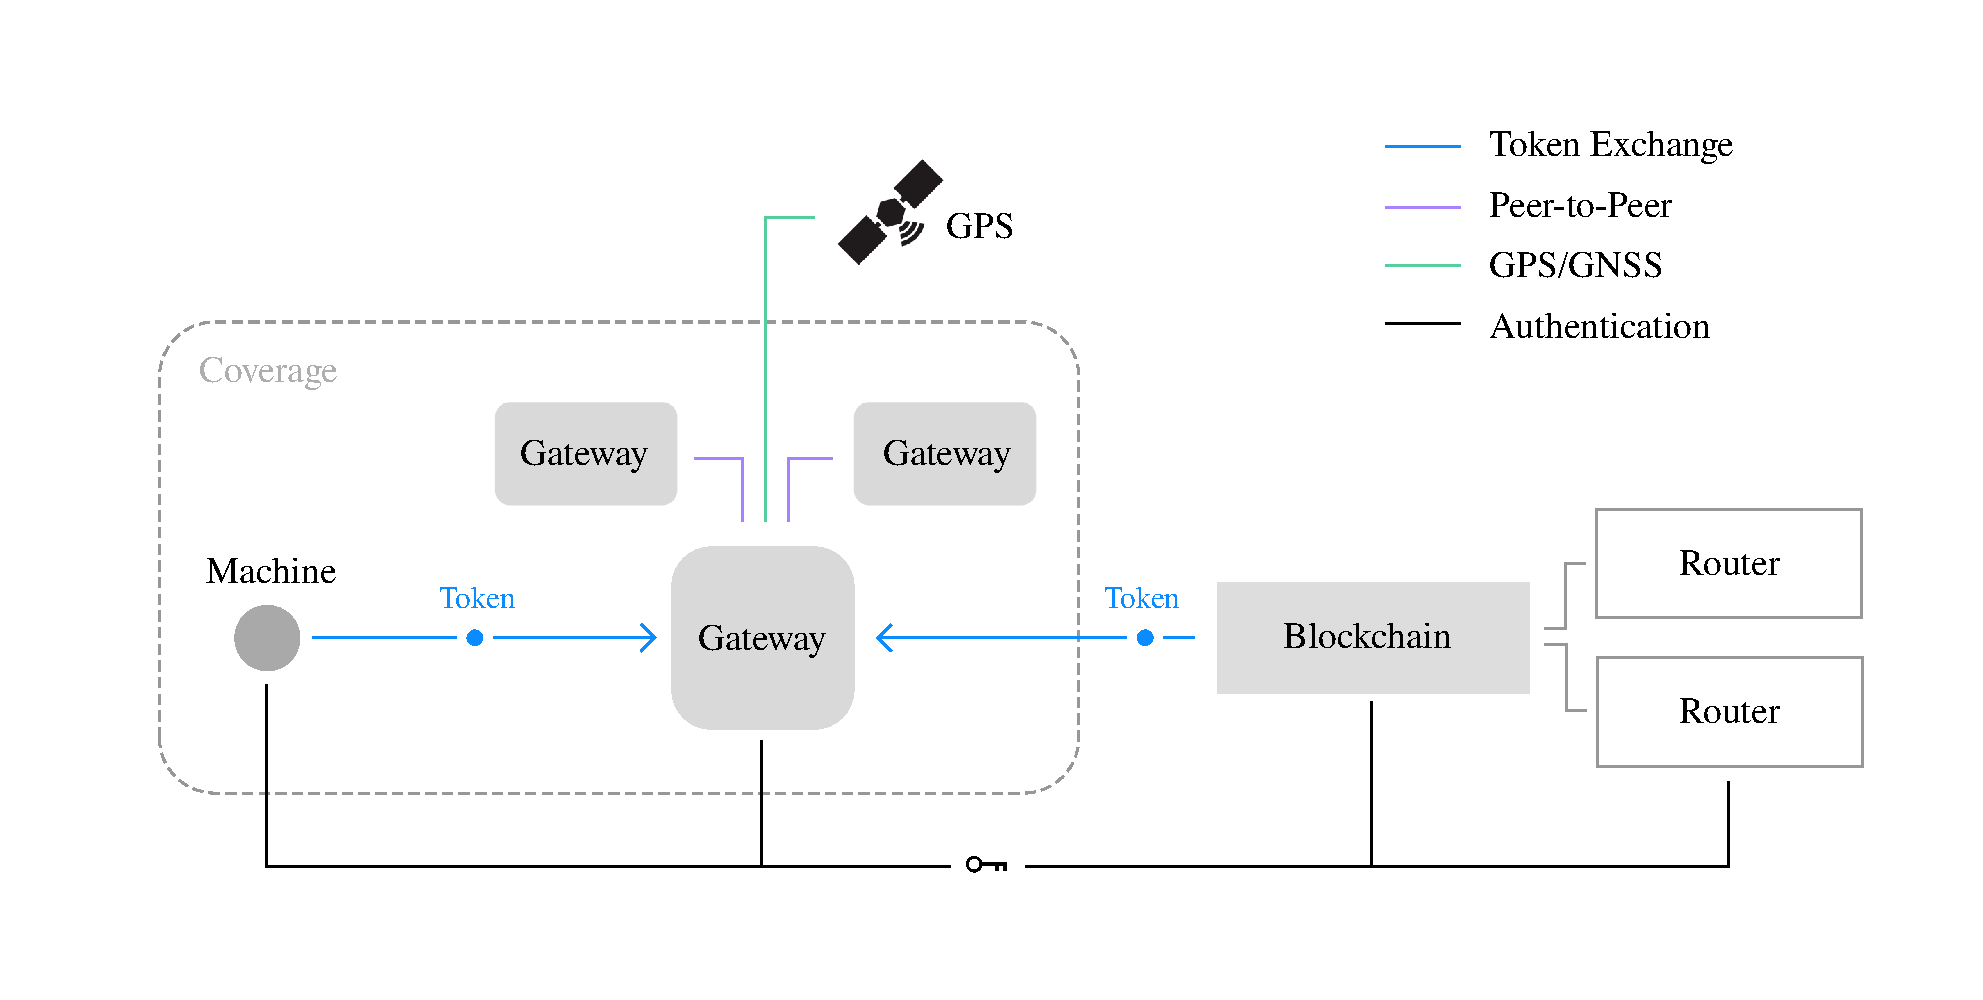
\includegraphics[width=\textwidth]{schematic.eps}
          \caption{\emph{System Overview}}
          \label{fig:system}
     \end{center}
\end{figure*}


\section{The Helium DMN}

We introduce the Helium Decentralized Machine Network (\verb|DMN|). The \verb|DMN| provides wireless access to the internet for devices by way of multiple independent miners, and outlines a network and wireless protocol specification by which participants in the network should conform. Devices pay this network of miners for sending data to and from the internet, and miners are rewarded with newly minted tokens for providing network coverage and delivering device data to the internet.

\subsection{Participants}

There are three types of participants in the network: Device, Miner, or a Router.

\begin{itemize}
    \item \emph{Devices} pay to send encrypted data to and from the internet via the \verb|DMN| using hardware compatible with the Helium wireless protocol, called \emph{WHIP} \secref{whip}. In locations with a sufficient number of miners, devices can pay several miners to geolocate themselves without needing satellite location hardware. Data sent from devices is \emph{fingerprinted}, and that fingerprint stored in the blockchain.
    \item \emph{Miners} provide wireless network coverage to the network via purpose-built hardware, called gateways \secref{gateways}, which provide a long-range bridge between WHIP devices and the internet. Users join the network as miners by purchasing or building a gateway that conforms to the wireless protocol, and \emph{staking} a token deposit proportional to the density of other miners operating in their area \secref{staking}. Miners participate in the \emph{Proof-of-Coverage} \secref{poc} process to prove that they are continuously providing wireless network coverage that devices can use. Miners join the network with a score \secref{scores} that diminishes as blocks pass without valid proofs being submitted. At a given epoch, a new group of miners are elected to a \emph{consensus group} which mine new blocks in the blockchain and receive the block reward and transaction fees for any transactions included in the block once mined. As a miners score drops their probability of being elected to the consensus group and mining blocks diminishes.
    \item \emph{Routers} are internet applications that receive encrypted device data from miners. Routers are the termination point for device data encryption. Devices record to the blockchain which routers miners should send their data to, such that any gateway on the network can send any devices data to the appropriate router. Routers are responsible for confirming to gateways that device data was delivered to the correct destination and that the miner should be paid for their service.
\end{itemize}

\subsection{Blockchain} \label{blockchain}

The Helium blockchain is a distributed ledger designed to provide a cost-effective way to run application logic core to the operation of a \verb|DMN|, store immutable device data fingerprints, and furnish a transaction system. The Helium blockchain is an immutable append-only list of transactions which achieves consensus by verifying \emph{Proofs-of-Coverage} \secref{poc}. Users internal and external to the \verb|DMN| have access to the blockchain, which is a new protocol built from scratch specifically for the \verb|DMN|.

$B$ consists of blocks $b_n$, which contain a header and a list of transactions. There are several kinds of transactions, outlined in \secref{transactions}. 

As in other implementations, $b_n$ consist of a hash of the previous block in the chain, a set of transactions, and a proof. At a given epoch $t$ a block $b_t$ consists of:

\begin{center}
    \begin{tabular}{|c|}
         \hline
         Block Version \\
         \hline
         Block Height \\
         \hline
         Previous Block Hash \\
         \hline
         Transactions \emph{1..n} Merkle Hash \\
         \hline
         \emph{Proofs-of-Coverage} \\
         \hline
         \emph{Proof-of-Serialization} \\
         \hline
    \end{tabular}
\end{center}

As the \emph{Proof-of-Coverage} \secref{poc} is valuable to the network, miners are required to submit their proofs at regular intervals. All miners have a score which decays over time, and is boosted by submitting \emph{Proofs-of-Coverage} to the blockchain. At a fixed epoch, a \emph{HoneyBadgerBFT} \cite{honeybadger} consensus group of the highest scoring miners is elected. For that epoch, all transactions are encrypted and submitted to the consensus group for inclusion in the blockchain. The consensus group is responsible for decrypting transactions using \emph{threshold decryption}, agreeing on the validity and ordering of transactions, forming them in to blocks, and appending them to the blockchain for which the members of the consensus group receive a reward.

As the consensus group is validating transactions prior to inclusion in the blockchain, there is practically no settlement time, and the transaction throughput is extremely high compared to a \emph{Nakamoto Consensus} blockchain such as Bitcoin or Ethereum. The Helium Consensus Protocol is outlined in detail in \secref{consensus}.

\subsection{Physical Implementation}

In addition to the blockchain network, Helium is a \emph{physical} wireless network instantiation. The participants in the wireless network can be thought of as follows:

\begin{description}
    \item [Wireless Protocol] The wireless network uses a new open wireless protocol, called \emph{WHIP}. WHIP is a long-range, low-power, wireless network protocol suitable for use with commodity open-standards hardware. WHIP compatible hardware can communicate over many square miles in dense urban environments or hundreds of square miles in rural settings. WHIP compatible hardware can also last for several years using standard batteries. WHIP uses strong public key cryptography and authentication occurs using the Helium blockchain, with end-to-end encryption.

    \item [Gateways] Gateways are physical network devices that provide wide-area wireless coverage and participate in the blockchain network. Gateways transmit data back and forth between routers on the internet and devices while generating \emph{Proofs-of-Coverage} for the blockchain network \secref{poc}. Gateways are manufactured using commodity open-standards components with no proprietary hardware. Gateways can cooperate and geolocate devices using the wireless network without any additional required hardware. Each Gateway can support thousands of connected devices, and provide coverage over many square miles. Miners operating gateways specify the price they are willing to accept for transport and \emph{Proof-of-Location} services for devices.

    \item [Devices] Devices exist in the form of hardware products that contain a WHIP-compatible radio transceiver and communicate with gateways on the wireless network. WHIP is designed to facilitate low power data transmission and reception, so typically devices exist in the form of battery-powered sensors that can oeprate for several years using standard batteries (although mains-powered devices also work quite well). Devices can exist in a variety of forms, depending on the product or use case, and a variety of transmission and reception strategies can be employed to optimize for transmission/reception frequency or battery life. Device manufacturers are encouraged to use hardware-based key storage which can securely generate, store, and authenticate public/private key pairs without leaking the private key.
\end{description}

In this section, we expand on the components of the wireless network.

\subsection{Wireless Protocol (\emph{WHIP})}\label{whip}

\begin{description}
    \item [Motivation] Several Low Power Wide Area Network (LPWAN) technologies are available today. These wireless technologies focus on creating extremely long-range, low-power internet communication for sensors and other smart devices. Typically these technologies trade throughput for range, with data rates as low as 18~bits~per~second (bps) and range measured in miles. In comparison, a typical WiFi network has significantly higher data rates but ranges limited to only a few hundred feet. Several of these new technologies, such as LoRa~\cite{lora} and RPMA~\cite{rpma}, have gained good traction and there are many commercial products available compatible with these systems. However, we believe a decentralized machine network should use non-proprietary protocols and modulation schemes and that participants in this ecosystem should have the freedom to choose between competing hardware vendors. We do not consider an open alliance built on top of proprietary hardware to be an acceptable compromise. While there are many open-standard wireless networking stacks, such as IEEE~802.15.4~\cite{ieee802_15_4} used in the first generation of Helium wireless products, none meet our extremely long range and low power criteria. It is this lack of open solutions that drove the creation of a new protocol.

    \item [Outline] We introduce a new open-source Low Power Wide Area Network (LPWAN) protocol called \emph{WHIP}. WHIP is a highly secure, long range, low power wireless network protocol that is compatible with a wide range of existing radio transceivers operating in the sub-GHz unlicensed frequency spectrum. Authentication with the wireless network uses modern public-key encryption and NIST~P-256 ECC key pairs, with the public keys for all participants stored in the blockchain.

    The modulation format is simple and widely supported, easy to implement and has excellent resistance to RF noise. There are dozens of vendors implementing radio transceivers compatible with WHIP, such as Texas Instruments, Microchip, and Silicon Labs.

    WHIP is a \emph{narrowband} wireless protocol which creates several channels within the unlicensed spectrum and employs frequency hopping to hop between channels. Typically frequency hopping requires a complex time-synchronized system that is limited in capacity. However, devices using WHIP do not need to coordinate with gateways on channel selection as gateways are capable of hearing all channels within the available spectrum at any time. We choose narrow-band to accomplish the following goals:

    \begin{description}
        \item[Spectral Efficiency] it is necessary to operate within unlicensed RF spectrum very efficiently. RF is a shared, limited resource, and therefore a focus on efficiency to increase capacity and improve robustness is a must.
        \item[Co-Existence Performance] as the number of devices and networks increase, the ability to operate in \emph{noisy} RF environments without interference is a critical consideration.
        \item[Range] narrowband allows for extremely long-range communications, with data rates that scale both up and down depending on the density of gateways.
    \end{description}

    \item [Implementation] WHIP supports several data rates, channel bandwidths, and error-correction techniques. Gateways and devices dynamically negotiate the combination of these options using a \emph{signalling packet} delivered at the lowest bandwidth and symbol rate to ensure maximum range for the initial communication.
\end{description}

The full WHIP specification will be made available by the Decentralized Machine Network Alliance.

\subsection{Gateways}\label{gateways}

Gateways are physical network devices operated by miners that create wireless RF coverage over wide areas. They transmit data back and forth between routers on the Internet and devices on the network, process blockchain transactions, and create \emph{Proofs-of-Coverage} for the blockchain network \secref{poc}. Gateways can connect to the Internet using any TCP/IP capable backhaul, such as Ethernet, WiFi or Cellular. Each gateway contains a radio frontend chip capable of listening to several MHz of radio spectrum at a time and can hear all network traffic transmitted within that spectrum. In this configuration modulation and demodulation is done in software, which is typically referred to as a \emph{Software Defined Radio (SDR)}. The benefit of this structure is that gateways can hear any device traffic transmitted within the frequency range, and no synchronization between the gateway and device needs to occur. This allows devices to remain inexpensive and relatively simple and reduces wireless protocol overhead. If a miner wishes to minimize their gateway hardware costs, synchronized frequency hopping schemes are also permitted within the specification as a cheaper alternative to a more expensive radio frontend.

Gateways require a GPS or GNSS receiver to obtain accurate position and date/time information. This satellite-derived location is used in conjunction with other techniques to verify that a gateway is, in fact, providing wireless network coverage in the location it claims. Because satellite location messages are easy to fabricate and do not necessarily prove that wireless RF coverage is being created, multiple mechanisms are required to validate this work as described in more detail in \secref{poc}.

Satellite location information is also correlated with packet arrival events to provide \emph{Time Differential of Arrival (TDoA)} location for devices if multiple gateways observe the same packet. This allows devices to locate themselves without requiring a GPS/GNSS transceiver physically, and therefore provide accurate location data at a fraction of the battery life and cost of competing methods. This method is described in detail in \secref{geolocation}.

Helium Systems Inc.\ will make both a complete open-source reference design and a finished product available for immediate participation in the network.

\subsection{Devices}\label{devices}

A \emph{device} is any wireless hardware capable of communicating with gateways on the network. WHIP is designed to facilitate low power data transmission and reception, so typically devices would exist in the form of battery-powered sensors that can function for several years using standard batteries.

WHIP is designed such that devices can be manufactured using commodity hardware available from a wide variety of vendors with a very low-cost bill of materials (BOM). The technology in modern radio transceivers, such as the Texas Instruments CC1125 or STMicroelectronics S2-LP, enables exceptionally long-range network systems that can be built without the need for proprietary modulation schemes or physical layers. Some of these radios are available for around \$1 at reasonable volumes.

It is recommended that each device use the Microchip ECC508A or equivalent hardware-based key storage device, which can securely generate, store, and authenticate public/private \emph{NIST P-256 ECC} \cite{nist} key pairs without leaking the private key. Also, a wide array of defense mechanisms prevent logical attacks on the encrypted data between the key storage device and its host device, along with physical protections on the security device itself. Users program their key storage device as part of the onboarding process defined in the WHIP wireless specification using a simple SDK\@.

\subsection{Routers}

Routers are internet-deployed applications that receive packets from devices via gateways and route them to appropriate destinations such as an HTTP or MQTT endpoint. Routers also act as \emph{full nodes} for the blockchain network \secref{full-nodes}.

Routers serve several functions on the network, including:

\begin{itemize}
    \item Authenticating devices with the wireless network
    \item Receiving packets from gateways and routing them to the Internet
    \item Delivering downlink messages, including OTA updates, to devices via gateways
    \item Providing delivery confirmations to ensure transport transactions are honest
    \item Providing authentication and routing mechanisms to third-party cloud services such as Amazon AWS or Microsoft Azure
    \item Storing and making available a full copy of the blockchain ledger
\end{itemize}

When a gateway receives a data packet from a device on the network, it queries the blockchain to determine which router to use given the device's network address. Anyone is free to host their own router and define their devices' traffic to be delivered there by any gateway on the network. This ability allows users of the network to create VPN-like functionality whereby encrypted data is delivered only to a router (or set of routers) that they specify and can optionally host themselves.

Routers can implement a system called a \emph{Channel} which handles the authentication and routing of data to a specific third party Internet application, such as Microsoft's Azure IoT Hub. These channel implementations can take advantage of a device's onboard hardware security to create a secure, hardware-authenticated connection to a third party which would otherwise be difficult to implement directly on an embedded microcontroller. Helium will make available an open source reference implementation of a Channel that can be used to build additional interfaces to Internet services.

Helium Systems Inc will also host a high-availability cloud router for anyone to use and also provides and maintains an open-source router that is available either as source code or a binary package for a variety of operating systems and distributions.

The protocol specification required for implementing a router is defined in the WHIP Wireless Specification document that will be made available by the Decentralized Machine Network Alliance.

\section{\emph{Proof-of-Coverage} \& \emph{Proof-of-Serialization}}\label{poc}

In the Helium network, miners must prove that they are providing wireless network coverage that devices are able to use to communicate with the internet. Miners do this by complying with the \emph{Proof-of-Coverage} protocol which the blockchain network and other miners audit and verify. We use a \emph{Proof-of-Serialization} to ensure that miners are correctly representing their time in relation to others on the network, and obtain cryptographic proof of dishonest behavior. Several components of the Helium network, such as blocks in the blockchain, use \emph{Proof-of-Serialization} as a cryptographic ``anchor'' that root those occurrences  with a cryptographic time proof. With a combination of \emph{Proof-of-Coverage} and \emph{Proof-of-Serialization} we can obtain cryptographic proof of the approximate location and time of events occurring within the Helium network.

In this section we outline the motivation and implementation for \emph{Proof-of-Coverage} and \emph{Proof-of-Serialization}.

\subsection{Motivation}

Most existing blockchain networks such as Bitcoin~\cite{bitcoin} and Ethereum~\cite{ethereum} use a \emph{Proof-of-Work} system that relies on an algorithmic puzzle that is asymmetric in nature. These proofs are extremely difficult to generate, but simple for a third party to verify. Security on these networks is achieved by the network-wide \emph{consensus} that the amount of computing power required to generate a valid proof is difficult to forge, and as subsequent blocks are added, the cumulative difficulty of the chain becoming prohibitively difficult to fabricate.

These computation-heavy proofs are, however, not otherwise \emph{useful} to the network. We define useful as work that is valuable to the network beyond securing the blockchain. While there have been attempts in other networks to turn mining power into something useful, such as Ethereum executing small programs, the majority of the work is not useful or reusable. The mining process is also extremely wasteful, as the determining factor in the work is typically computational power which consumes massive amounts of electricity and requires significant hardware to execute.

The proofs used in Helium must be resistant to \emph{Sybil Attacks} in which dishonest miners create pseudonymous identities and use them to subvert the network and gain access to block rewards to which they should not be entitled. This is a particularly difficult attack vector to manage in a physical network like Helium. We must also be resistant to a new attack vector: \emph{Alternate Reality Attacks} exist where a dishonest group of miners are able to simulate that wireless network coverage exists in the physical world when it in fact does not. An example of this would be running the mining software on a single computer and simulating GPS coordinates and RF networking.

We later propose a consensus protocol \secref{consensus} that uses \emph{Proof-of-Coverage} to both secure the blockchain and provide an extremely useful service to the network; providing wireless network coverage that devices can use to send data to and from the Internet.

\subsection{Inspiration}

\emph{Proof-of-Coverage} (\verb|PoC|) is an innovative proof which allows miners to prove that they are providing wireless network coverage $W$ in a specific region to a challenger, $C$. \verb|PoC| is an interactive protocol where a set of targets $T_n$ assert that $W$ exists in a specific GPS location $L$ and then convinces $C$ that $T_n$ are in fact creating $W$ and that said coverage must have been created using the wireless RF network. \verb|PoC| is the first such protocol that attempts to prove the veracity of miners in a physical space, and then use it to achieve consensus on a blockchain network.

With \verb|PoC| we aim to solve for the following:

\begin{itemize}
    \item Our goal is to prove that miners are operating radio frequency (RF) hardware and firmware compatible with the wireless protocol
    \item Our goal is to prove that miners are located in the geography they claim by having them communicate via RF
    \item Our goal is to correctly identify which version of reality is correct when there is a conflict
\end{itemize}

\emph{Proof-of-Coverage} is inspired by the \emph{Guided Tour Protocol (GTP)}~\cite{gtp} which devises a system for denial of service prevention by requiring a client $c$ to make a request to a variety of ``tour guide'' computers $G_n$ in order to gain access to a server $s$. The tour guides must be visited in a specific order and a hash of data exchanged which reveals the location of the next $G_n$ in order. Only after every $G_n$ has been visited can $c$ gain access to $s$.

Once $c$ gets to the last stop of the tour, it submits evidence of the first and last stop to $s$ who is able to verify that the first and last stops of the tour are correct without needing to contact $G_n$, and that $c$ could only know the first and last stops if it had completed the tour correctly.

While an extremely clever and innovative system, GTP is not directly suitable as a proof in our wireless network as radio frequency (RF) networking has limited range and therefore cannot communicate with peers anywhere on the network. We aim to construct a proof loosely based on the ideas presented in GTP, but applicable to our protocol.

We combine \emph{Proof-of-Coverage} with \emph{Proof-of-Serialization}---a proof that allows miners on the network to achieve cryptographic time consensus among decentralized clients. We aim to achieve rough time synchronization in a secure way that does not depend on any particular time server, and in such a way that, if a time server does misbehave, clients end up with cryptographic proof of that behavior.

\subsection{Constructing \emph{Proof-of-Coverage}}

This section describes the construction of the \emph{Proof-of-Coverage} protocol.

We aim to construct a proof that takes advantage of the following characteristics of radio frequency (RF) communication that are unique and different to internet communication:

\begin{enumerate}
    \item RF has limited physical propagation and therefore distance
    \item RF travels at the speed of light with (effectively) no latency
\end{enumerate}

Our goal is to verify whether miners in a physical region are acting honestly and creating wireless network coverage compatible with the Helium wireless protocol (WHIP). To do this, a challenger $C$ deterministically constructs a multi-layer data packet $O$ which begins at an initial target, $T_1$, and is broadcast wirelessly to a set of sequential targets, $T_n$, each of which are only able to decrypt the outer-most layer of $O$ if they were the intended recipient. Each target signs a receipt, $K_s$, delivers it to $C$, removes their layer of $O$, and broadcasts it for the next target. Essentially, an ``envelope of envelopes'' only decipherable by the intended recipient.

\begin{figure}[ht]
    \begin{center}
          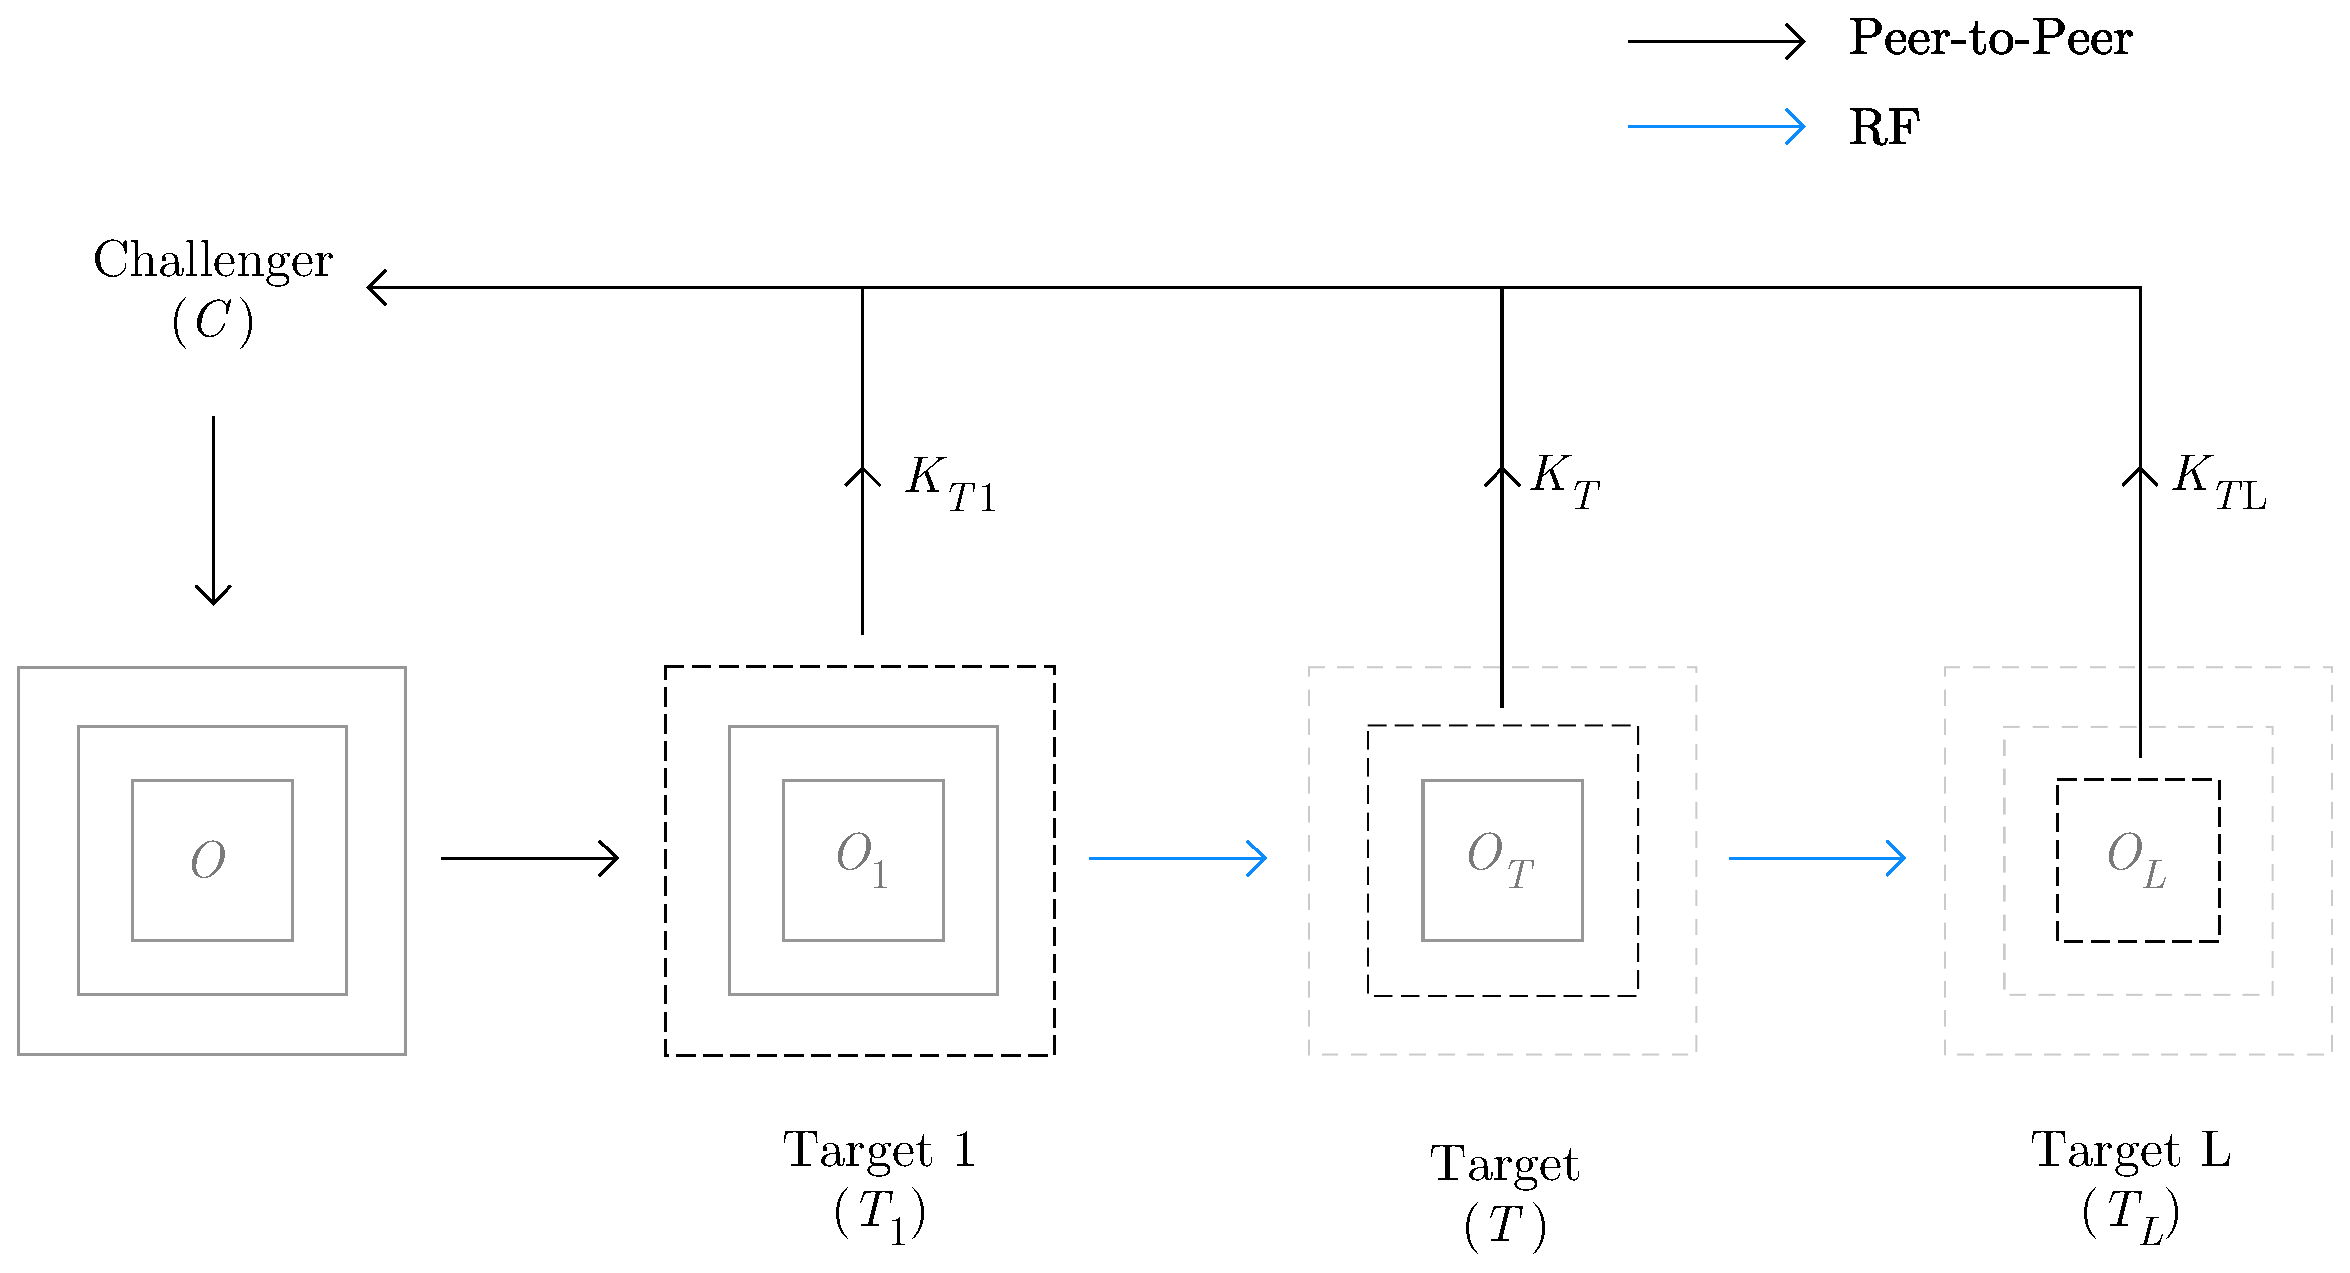
\includegraphics[width=\columnwidth]{deconstruction.eps}
          \caption{\emph{Multi-Layer Data Packet Deconstruction}}
          \label{fig:poc-deconstruction}
     \end{center}
\end{figure}

\textbf{Selecting the Initial Target}. We aim to deterministically locate a geographic reference target, $T$, for the challenger, $C$. Both $C$ and $T$ are miners in the network. $T$ does not need to be geographically proximate to $C$. To locate $T$, $C$ uses a \emph{consistent hash ring} $\omega$, of potential miners. $\omega$ only contains miners eligible as targets as described in \secref{mining}, and miners are allocated portions of $\omega$ that are inversely proportional to their score, increasing the probability of potentially dishonest miners being targeted. We refer the interested reader to \cite{hashing} for further reading on consistent hashing techniques. Given that a miners score is diminishing linearly over time \secref{scores}, it is necessary to create this inverse relationship to give low-scoring miners an opportunity to participate in the process and increase their score. This diminishing score also incentivizes all the participants to send receipts to the challenger and broadcast the remainder of $O$. $C$ seeds verifiable entropy, $\eta$, into the selection process by signing the current block hash with their private key.

\textbf{Constructing the multi-layer challenge}. Once $T$ has been selected, $C$ must construct a multi-layer challenge, $O$. $O$ is a data packet broadcast over the wireless network and received by geographically proximate targets $T_n$. Geographically proximate is defined as within a radius of $T$, a network value $T$\textsubscript{radius}. Each layer of $O$, $O_l$, consists of a three-tuple of $E\left(S, \psi, R\right)$, where $E$ is a secure encryption function using the ECDH derived symmetric key, $S$ is a nonce, $\psi$ is the time to broadcast the next layer of the challenge and $R$ is the remainder of $O$ consisting of recursive three-tuples. The maximum number of $O_l$ is bounded by a network value, $O$\textsubscript{max}.

The construction logic of $O$ by $C$ is as follows:

\begin{enumerate}
  \item A set of candidate nodes, $T_n$, are selected such that all members of $T_n$ are within a contiguous radio network that also contains $T$
  \item Two targets, $T_1$ and $T_L$, are selected by finding the highest scoring targets in $T_n$ furthest from $T$
  \item A weighted graph, $T_g$, is constructed from $T_n$ such that members of $T_g$ in radio range of each other are connected by an edge weighted by the value of \(1 - \Big({score(T_a) - score(T_b)}\Big)\)
  \item The shortest path between $T_1$ to $T$ to $T_L$ is computed using Dijkstra's algorithm\cite{dijkstra} using the edge weights from the previous step
	\item An ephemeral public/private keypair $E_k$ and $E$\textsubscript{k-1} are generated
	\item A layer $O_l$ is created and added to $O$, and $S$ is encrypted with the combination of the public key of $T_L$, retrieved from the blockchain as $T_L$$_k$ and $E$\textsubscript{k-1} as an Elliptic-Curve Diffie-Hellman (ECDH) exchange to compute a shared secret, known only to both parties $C$ and $T_L$
  \item The previous step repeats with additional layers added to $O$ until all $T_L$ $\rightarrow$ $T_1$ have a layer $O_l$ included in $O$
\end{enumerate}

The resulting $O$ can be visually represented as depicted in \figref{fig:poc-o_construction}.

\begin{figure}[ht]
    \begin{center}
          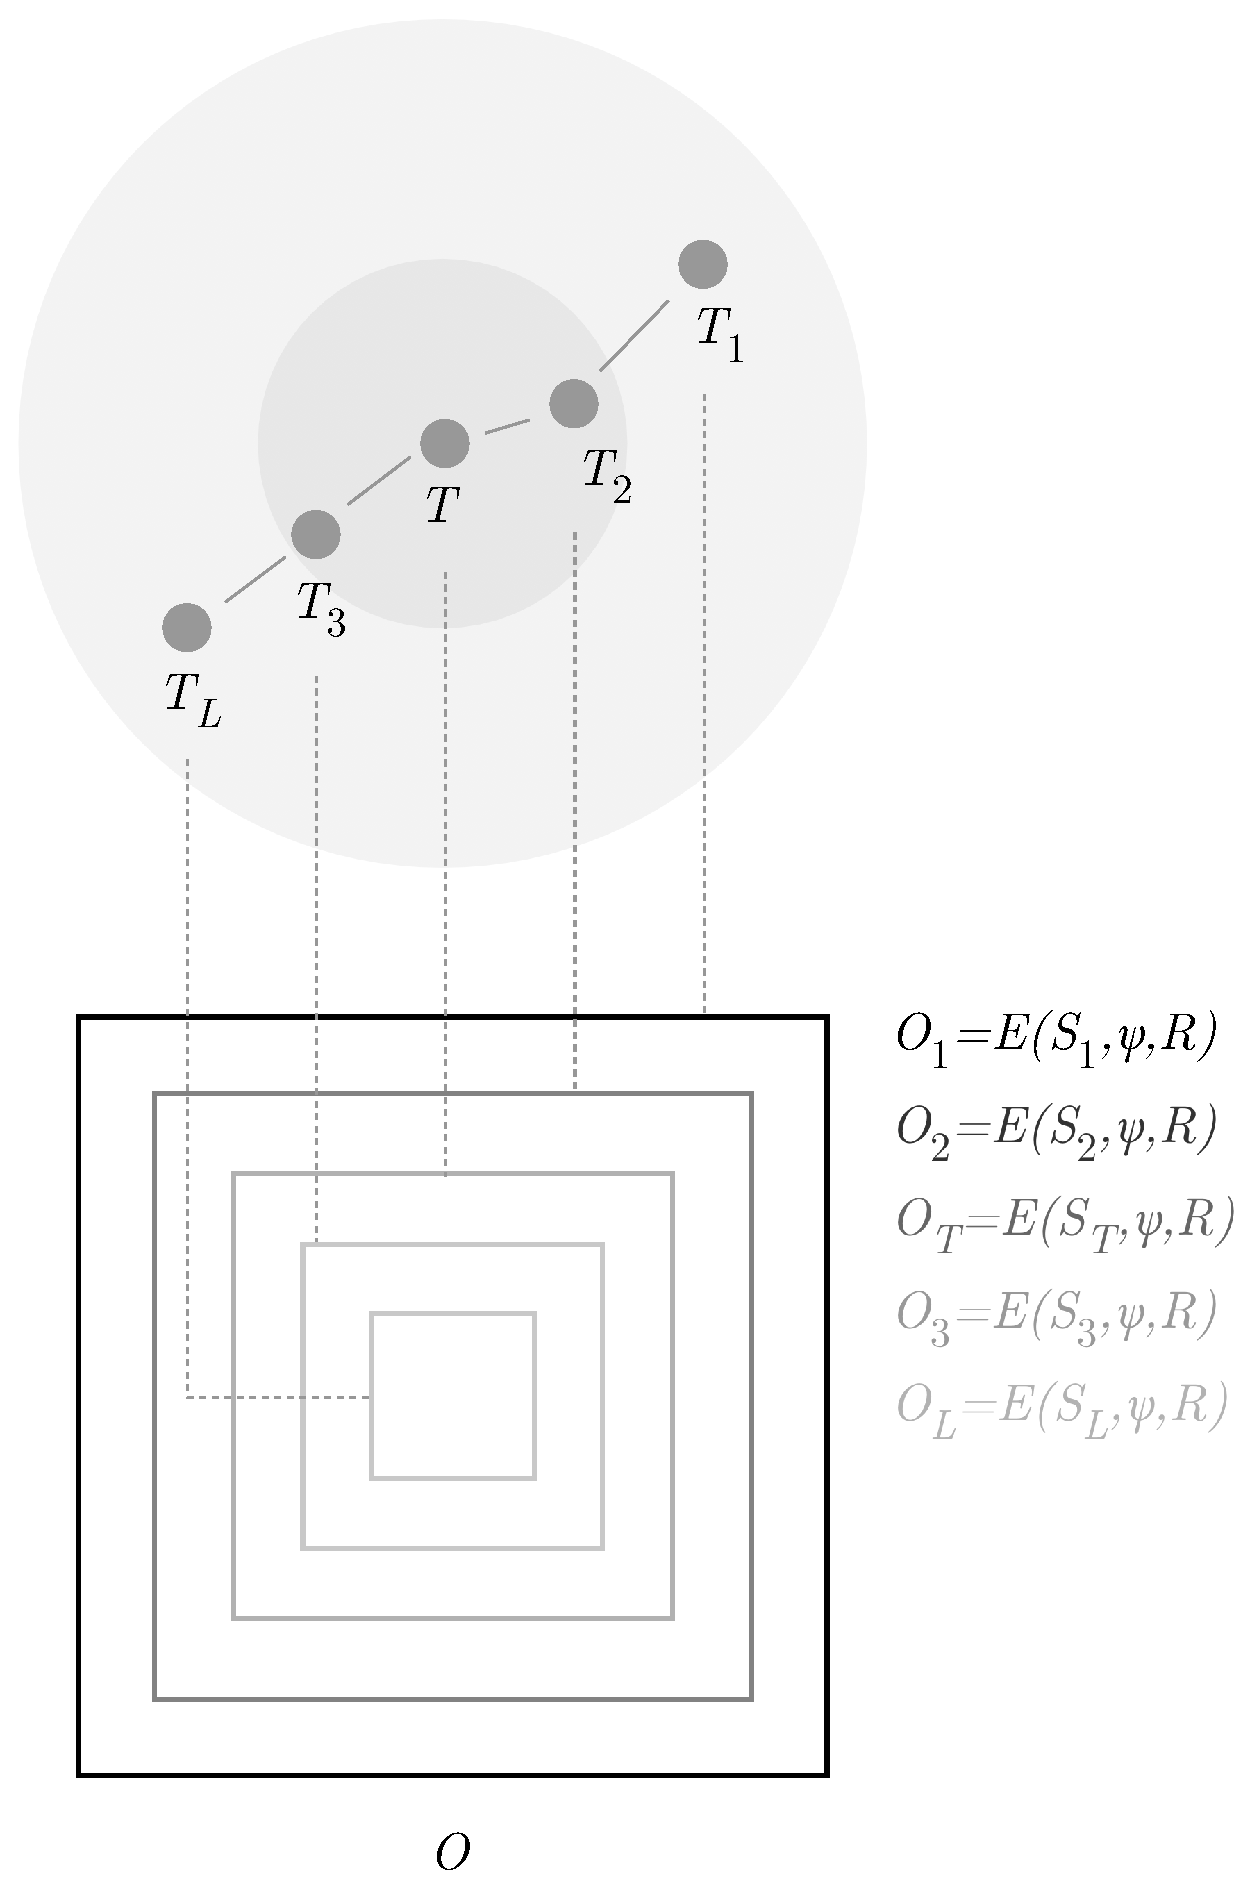
\includegraphics[width=\columnwidth]{o_construction.eps}
          \caption{Construction of $O$}
          \label{fig:poc-o_construction}
     \end{center}
\end{figure}

\textbf{Creating the Proof}. Once $O$ has been constructed, it is delivered to $T_1$ via the internet peer-to-peer network and immediately broadcast via the wireless network. The Helium wireless protocol is not a point-to-point system, so several miners within proximity of $T_1$ will hear $O$. As described prior, each layer $O_l$ of $O$ contains the three-tuple ${E\left(S, \psi, R\right)}$ where $E$ is a secure encryption function using the ECDH-derived key, $S$ is a nonce, $\psi$ is a time at which to transmit the next layer of the packet and $R$ is the remainder of $O$ consisting of recursive three-tuples. In this example, only the specific target $T$ will be able to decrypt $E$ and send a valid receipt back to the challenger, $C$.

We describe the approximate flow of \emph{Proof-of-Coverage} creation as follows:

\begin{enumerate}
  \item $T_1$ receives $O$ from $C$ via the peer-to-peer internet network, decrypts the outermost layer and immediately broadcasts it $R$ via the wireless network
  \item $T$ hears $O$ and attempts to decrypt the value of $E$ by using its private key $pk:\ E_{pk}\left(S, \psi, R\right)$
  \item $T$ records both the time of arrival $\beta$ and the signal strength $\upsilon$ of $O$
  \item If successful, $T$ then creates signed receipt $K_s$, \\${K_s = \left(S || \beta || \upsilon\right)}$ signed by the private key of $T$
  \item $T$ submits $K_s$ to $C$ via the peer-to-peer internet network, removes the outer most layer, and wirelessly broadcasts the remainder $O$
  \item These steps repeat for $T_1$..$T$..$T_L$, with $T_L$ being the last target in the graph
\end{enumerate}

$C$ expects to hear responses from $T_g$ within a time threshold $\lambda$, otherwise it considers the \emph{Proof-of-Coverage} to have concluded. Because $C$ is the only party with complete knowledge of $O$, upper bounds of the values for $\beta$ and $\upsilon$ are assigned by $C$ which are used to verify that each layer of $O$ was transmitted approximately where and when it was expected. The upper bound for $\beta$ ls limited by the speed of light $\tau$ between $T_n$ and $T_n-1$. Thus we know that, subject to some slight delays from reflection or multipath, the packet should not arrive at $T_g$ later than $\tau$ multiplied by the geographical distance $D$ plus some small episilon value, $\upsilon = \tau \times \Big(D + \epsilon\Big)$. For $\upsilon$, because of the inverse-square law, we can calculate the maximum RSSI possible for a packet transmitted, $\mu$, from $T_g-1$ to $T_g$ as $\mu = \frac{1}{D^2}$. Gateways that are closer than expected, or which are transmitting at a higher power to mask their location disparity, are unlikely to get $\mu$ correct, given that they do not know who the next layer of $O$ is addressed to.

Once $T_L$ has delivered receipt to $C$, or $\lambda$ has elapsed, the \emph{Proof-of-Coverage} is completed. The collection of signed receipts, $K_s$, constitute the \emph{Proof-of-Coverage} that $C$ will submit to the network.

\begin{figure}[ht]
    \begin{center}
          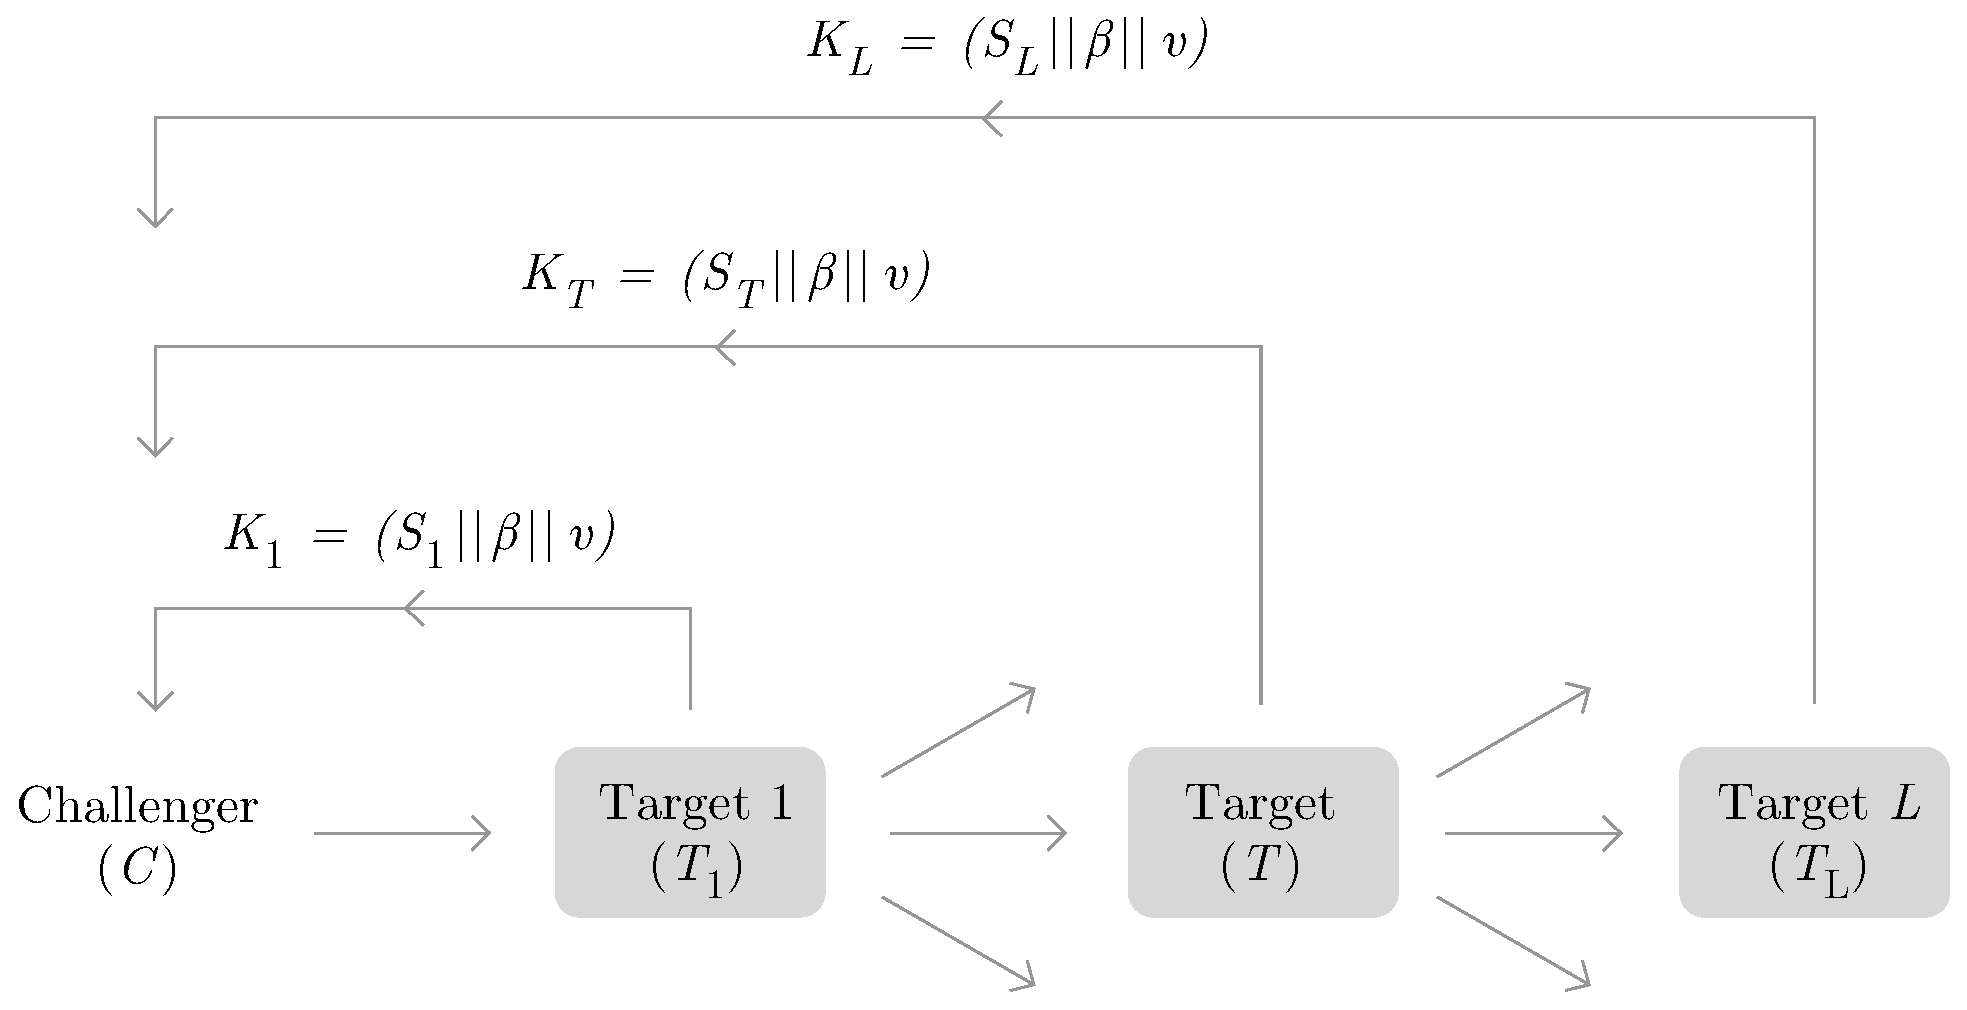
\includegraphics[width=\columnwidth]{o_propagation.eps}
          \caption{\emph{Proof-of-Coverage} flow}
          \label{fig:poc-propogation}
     \end{center}
\end{figure}

\textbf{Scoring} \label{scores} The score allocated to a miner, and therefore the resulting score of the \emph{Proof-of-Coverage}, is an integral part of the consensus protocol, further outlined in \secref{consensus}. When miners join the Helium network, they are assigned a score, $\phi_m$, with a value of \textbf{0.500}. We consider any miner with a score greater than 0.500 to be an honest miner, $\eta$. This score depreciates according to the number of verifications the miner has as well as the height since their last successful verfication. As $\phi_m$ decreases the probability of the miner $M$ being the target for $C$ increases such that the network continually attempts to prove that the lowest scoring miners are acting honestly, and giving miners a reasonable chance to improve their score.

In order to achieve such behavior we define the following invariants:

\begin{tabular}{l l}
        $M$, & miner                                         \\
        $v$, &number of successful verfications for $M$ -\\
        & number of failed verifications for $M$ \\
        $h$,          & height since the last successful verification for $M$\\
\end{tabular}

If we assume that the ideal verification interval for any miner is close to 240 blocks (4 hours if we assume a 60 second block time), we scale the defined invariants to fit the scoring functions:

\begin{tabular}{l l}
        $v'$, &$v/10.0$\\
        $h'$, &$h/480$ \\
\end{tabular}

Using the above we can now construct a staleness-factor, $\delta$, which would be used in determining the score of the miner $M$.

\begin{equation*} \label{score}
        \delta{m} = \begin{cases}
        	-(8.h')^{2}&\text{$v'$ = 0}\\
        	v'.(1 - \frac{h'^{2}}{min(0.25, v')})&\text{$v'$ $>$ 0}\\
        	v'.(1 - 10.v'.h'^{2})&\text{$v'$ $<$ 0}
        \end{cases}
\end{equation*}

The above conditions strictly adhere to the following principles:

\begin{enumerate}
  \item A negative $v$ indicates that the miner is consistently failing verification.
  
  \item If $v$ = 0, we don't have any trust information, therefore, we use a steep parabolic curve for the decay dependent on $h'$.
  
  \item If $v$ $>$ 0, it implies that the miner has been successfully verified consistently, hence, we use an inverse parabolic curve that crosses the Y axis at 1, where the width of the parabola increases as a factor of $v$ up to 0.25. This implies that the more positive verifications\secref{poc} the miner has accrued, the slower its score decays as a factor of $h'$.
   
  \item Finally, if $v$ $<$ 0, this is the inverse of the above case, wherein, a miner has consistently been failing verification. Therefore, we use a similar parabola as above, however, the width of the parabola decreases as a factor of $v$, leading to a higher score decay for the miner as a factor of $h'$.
  
\end{enumerate}

The following graph shows the trends for each of the above functions:

\begin{figure}[ht]
    \pgfplotsset{width=7cm, compat=newest}
    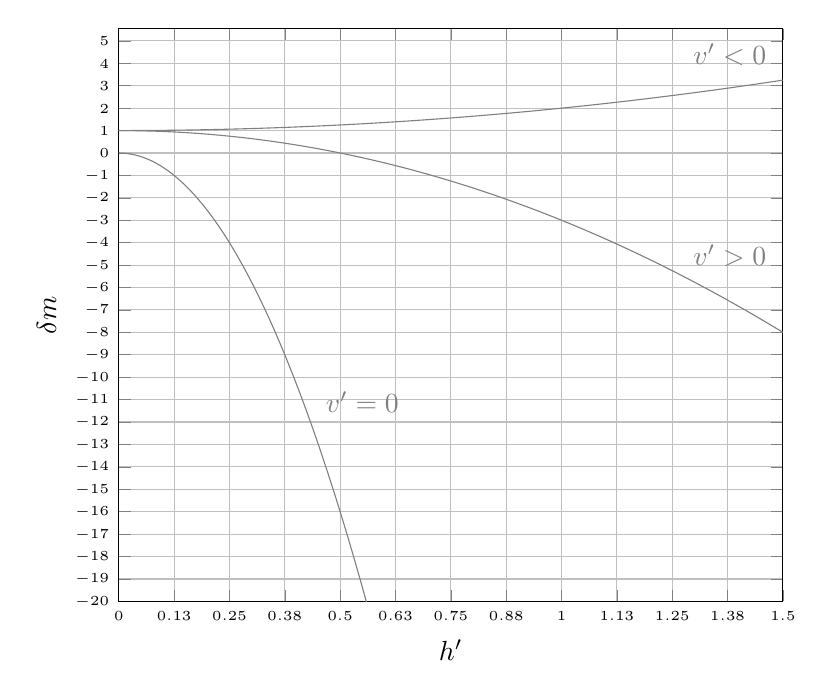
\begin{tikzpicture}
        \begin{axis}[xlabel = $h'$,
        ylabel = $\delta{m}$,
        xmin=0,
        xmax=1.5,
        ymin=-20,
        xtick={0, 0.125,...,1.5},
        ytick={-20, -19,...,5},
        scale only axis,
        grid=major,
        tick label style={font=\tiny}]
            \addplot[smooth, color=gray, samples=500]{-(8*x)^2};
            \node [anchor=south, color=gray] at (axis cs:0.55, -12)  {$v'=0$};
            \addplot[smooth, color=gray, samples=500]{1 -((x)^2)/0.25};
            \node [anchor=south, color=gray] at (axis cs:1.38, -5.5)  {$v'>0$};
            \addplot[smooth, color=gray, samples=500]{1 +((x)^2)};
            \node [anchor=south, color=gray] at (axis cs:1.38, 3.5)  {$v'<0$};
        \end{axis}
    \end{tikzpicture}
    \caption{\emph{Trendlines for the scoring functions}}
    \label{fig:score-trends}     
\end{figure}

Adhering to the above set of rules, we define the following scoring function, which is essentially a variation of a sigmoid curve fluctuating between values (0, 1):

\begin{equation*} \label{score}
        \phi_m = \frac{\arctan(2.\delta{m}) + 1.58}{3.16}
\end{equation*}

This scoring function yields the below graph, which shows the variation of the score with the staleness-factor:

\begin{figure}[ht]
    \pgfplotsset{width=7cm, compat=newest}
    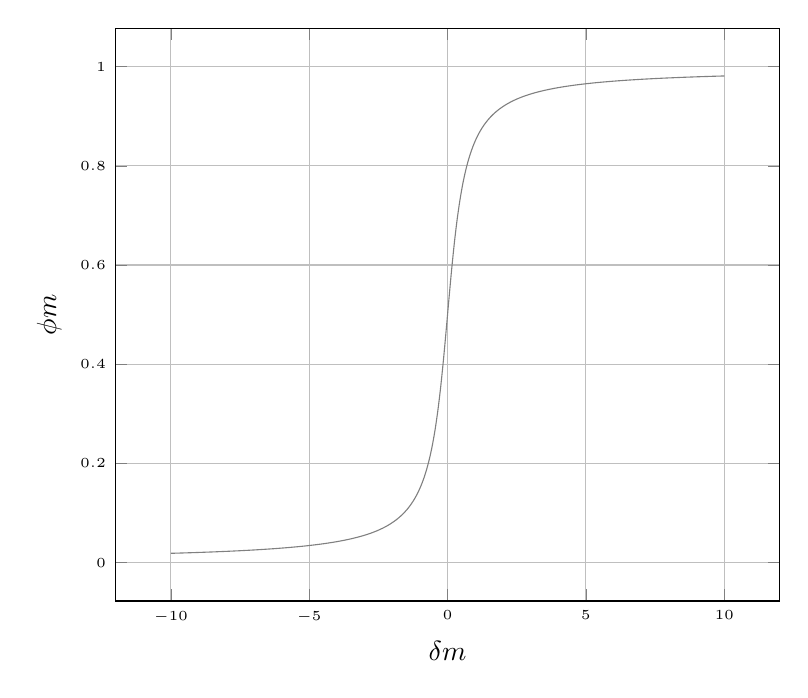
\begin{tikzpicture}
        \begin{axis}[xlabel = $\delta{m}$, ylabel = $\phi{m}$,
        scale only axis,
        grid=major,
        tick label style={font=\tiny}]
            \addplot[smooth, color=gray, domain=-10:10, samples=200]{(1.58 + rad(atan(2*x)))/3.16};
        \end{axis}
    \end{tikzpicture}
    \caption{\emph{Scoring algorithm and the resulting staleness factor}}
    \label{fig:score-stale}
\end{figure}

\figref{fig:score-graph} shows a snapshot of a random subset of the network at any blockchain height \textit{h}. The miners represent random locations with an illustrated score, while the edges are calculated using Dijkstra's algorithm\cite{dijkstra}.

\begin{figure}[ht]
    \begin{center}
          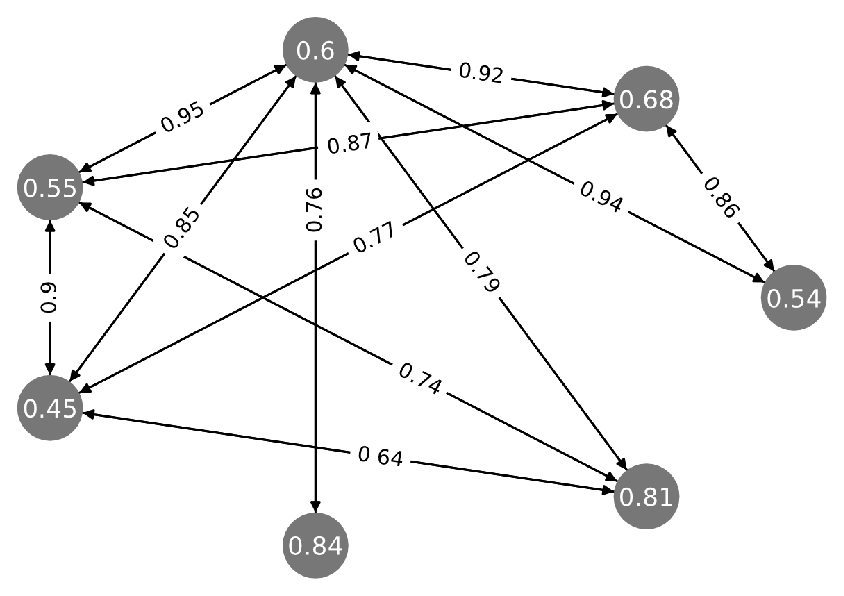
\includegraphics[width=0.8\columnwidth]{chart.eps}    
          \caption{\emph{Snapshot of a random subset of the initial network}}
          \label{fig:score-graph}
     \end{center}
\end{figure}

After 10,000 iterations the network appears as represented in \figref{fig:score-graph10000}.

\begin{figure}[ht]
    \begin{center}
          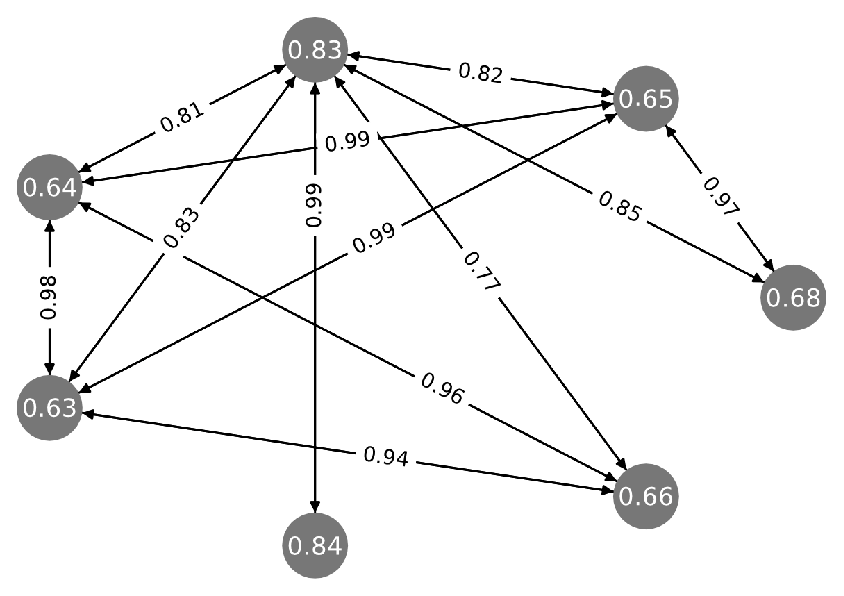
\includegraphics[width=0.8\columnwidth]{chart1000.eps}
          \caption{\emph{Snapshot of a random subset of the network after 10000 iterations}}
          \label{fig:score-graph10000}
     \end{center}
\end{figure}

The goal of this system is to ensure that the scoring algorithm considers that some miners may attempt to act dishonestly. However, because the calculated edge-weights (via Dijkstra's algorithm) and the target selection mechanism ensure that we only boost the score of a miner when it is being verified by other high scoring miners, we believe that the system will favor legitimate miners and deter dishonest ones.

\textbf{Target Selection}. Due to the way scoring decays, there is a possibility that a given miners' score may become stale as that miner may not be verified within a reasonable interval. We therefore structure the target selection mechanism to give miners a statistically greater chance to increase their score by being selected as a target as their score decays. This is accomplished by biasing the probability of miners being selected as potential targets based on their individual scores.

Let the set of miners be defined as:
\begin{equation*} \label{set-of-miners}
        N = \{m_1, m_2, m_3 \dots\ m_n \mid n > 1\}
\end{equation*}

Let the set of miner scores be defined as:
\begin{equation*} \label{set-of-scores}
        S = \{\phi_m, m \in N\}
\end{equation*}

We assign the target selection probability to each miner in the following way:
\begin{equation*} \label{target-selection-probability}
        P(m) = \frac{1-\phi_m}{n - \displaystyle\sum_{i=1}^{n} {\phi_{m_i}}}
\end{equation*}

The above equation ensures that the miner with the lowest score is assigned the highest probability of being selected as a potential target while the opposite holds for the miner with the highest score.

Furthermore, it also asserts that the probabilities are inversely proportional to the score of an individual miner. This allows us to successfully target potentially low scoring miners and improve the overall balance of the scoring system.

\textbf{Verifying the Proof}. Once $T_L$ has delivered $K_s$, or $\lambda$ has elapsed, the \emph{Proof-of-Coverage} is considered complete. When $C$ submits this proof, via a special type of transaction, all receipts $K_s$ from $T_1$...$T_L$ are included in the transaction published to the blockchain network. As all the steps originally completed by $C$ are deterministic in nature with verifiable and recreatable randomness, it is simple for a verifying miner, $V$, to recreate the original steps and verify that the proof is legitimate.

Verifying miners in the consensus group \secref{consensus} who see the proof transaction are able to verify the \emph{Proof-of-Coverage}by recreating the following steps:

\begin{enumerate}
        \item The verifying miner, $V$, reconstructs the hash ring of miners $\omega$
        \item The random seed $\eta$ can be verified by $V$ to have been created at approximately the correct time by the private key of $C$
        \item $V$ then selects $T$ from $\omega$, as seeding with $\eta$ will result in the same target selection
        \item The set of candidate $T_n$ are reconstructed from which $T_1$ and $T_L$ are determined
        \item Dijkstra's algorithm is used to reconstruct the graph $T_g$
        \item The $K_s$ receipts contained in $B_C$ are verified to have been signed by the private keys of $T_1$..$T$..$T_L$
\end{enumerate}

Assuming these steps are completed successfully, the \emph{Proof-of-Coverage} is verified the score of $C$ is adjusted appropriately.

\subsection{Constructing \emph{Proof-of-Serialization}}

To achieve cryptographic time consensus among decentralized clients, we implement a simplified form of Google's Roughtime \cite{roughtime}. Roughtime is a protocol that aims to achieve roughtime synchronization in a secure way that does not depend on any particular time server, and in such a way that, if a time server does misbehave, clients end up with cryptographic proof of that behavior.

This section describes the construction of the \emph{Proof-of-Serialization} protocol.

\textbf{Creating the Proof}. We outline the approximate process to achieve cryptographically secure time as follows:

\begin{enumerate}
        \item To begin, a miner $M$ pseudo-randomly picks two miners $M_1$ and $M_2$, to prove contact serialization with
        \item It is assumed $M$ has a public key for $M_1$ and $M_2$, otherwise $M$ should obtain it from the blockchain
        \item $M$ generates a nonce, $R$, which is a SHA512 hash of the block which $M$ has partially constructed
        \item $M$ then generates a salted hash commitment $K$ called the \emph{proof-kernel} ${K = H\left(R || M_1 || M_2\right)}$
        \item $M$ sends $K$ to $M_1$. $M_1$ replies with $T$, a signed message including the current time $T_1$ and $K$
        \item $M$ knows that the reply from $M_1$ was not pre-generated because it includes the nonce $R$ that $M$ generated
\end{enumerate}

Because $M$ can not trust $M_1$ it will ask for another time from $M_2$:

\begin{enumerate}
        \item For the second request, a new nonce $R$ is generated using $T$ truncated to 512-bits, blinded by XOR'ing a randomly generated 512-bit number
        \item $M$ then generates a sub-proof-kernel, $L = H\left(R || T || K\right)$, and sends it to $M_2$
        \item $M_2$ replies with $U$, a signed message including the current time $T_2$ and $L$
        \item $U$ is now a proof artifact that shows that $M$ desired and then proved a serialization between $M_1$ and $M_2$
\end{enumerate}

With only two servers, $M$ can end up with proof that something is wrong, but no idea what the correct time is. But with half a dozen or more independent servers, $M$ will end up with chain of proof of any server's misbehaviour, signed by several others, and enough accurate replies to establish what the correct time is, $T_t$.

\begin{figure}[ht]
    \begin{center}
          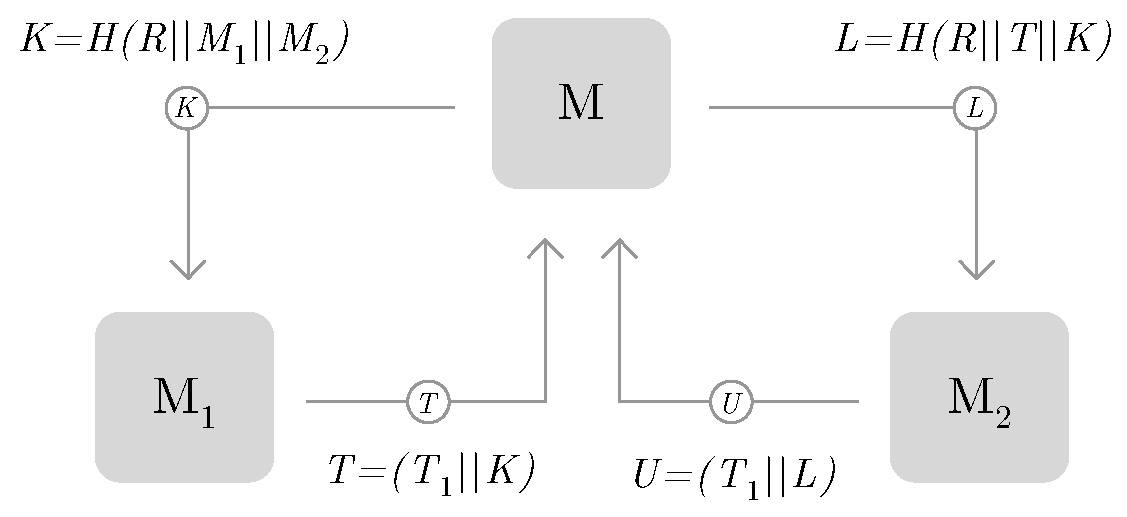
\includegraphics[width=\columnwidth]{serialization.eps}
          \caption{\emph{Creating Proof-of-Serialization}}
          \label{fig:serialization}
     \end{center}
\end{figure}

\textbf{Verifying the Proof}. If we assume that the times from $M_1$ and $M_2$ are significantly different, and the time from $M_2$ is before $M_1$, then $M$ has proof of misbehaviour. The reply from $M_2$ implicitly shows that it was created later because of the way that $M$ constructed the nonce. If the time from $M_2$ is after, then $M$ can reverse the roles of $M_1$ and $M_2$ and repeat the process to obtain, assuming steady clocks, a misordered proof as in the other case.

To verify the correct time, it is necessary for $M$ to repeat the time synchronization process with enough miners to gain consensus on the correct time:

\begin{enumerate}
    \item A miner $M$ again pseudo-randomly selects $n$ miners $M_1$...$M_n$
    \item $M$ generates a salted hash commitment $K$ and delivers it to $M_1$, where ${K = H\left(R || M_1 || M_2\right)}$
    \item $M_1$ again responds with $T$, a signed message containing the current time $T_1$ and $K$
    \item $M$ generates a sub-proof-kernel, $L = H\left(R || T || K\right)$, and sends it to the next miner $M_n$
    \item The next miner replies with $U$, a signed message including the current time and $L$
    \item These steps repeat through $M_n$ until at least three time responses, $T_n$, are monotonic
    \item $T_n$ can then be confirmed to be $T_t$, the correct time
\end{enumerate}

\begin{figure}[ht]
    \begin{center}
          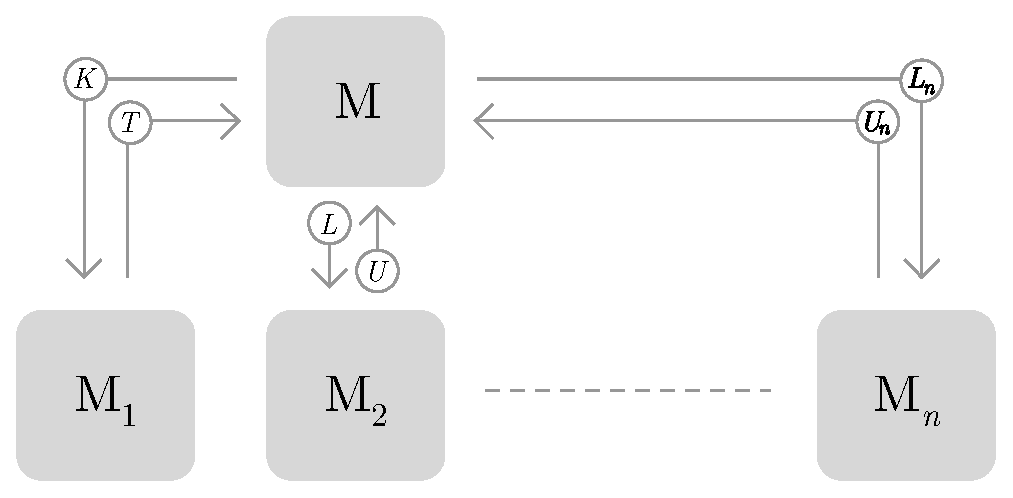
\includegraphics[width=\columnwidth]{verify_serialization.eps}
          \caption{\emph{Verifying Proof-of-Serialization}}
          \label{fig:verify-serialization}
     \end{center}
\end{figure}

\textbf{Utilizing the Proven Time}. Once the correct time $T_t$ has been determined via \emph{Proof-of-Serialization}, it is used by $M$ and included during block construction as described in \secref{blockchain}. The randomness $\eta$ used to compute $O$ and thus obtain the \emph{Proof-of-Coverage} is tied to the previous block, which contains $T_t$. This allows us to prove, with relative certainty, that some piece of data $D$ was created between the time of the previous block $b_t$ and $T_t$. $D$ in this case is the \emph{Proof-of-Coverage}. Thus we know that $D$ must have been constructed between $b_t$ and $T_t$. This ensures that the \emph{Proof-of-Coverage} cannot be pre-computed and that that blocks in the blockchain must have a minimum spacing in time; the \emph{blocktime}. Blocks which do not have at least \emph{blocktime} distance in time from their parent block are considered invalid.

\section{\emph{Proof-of-Location}} \label{geolocation}

Using \emph{Proof-of-Coverage} and \emph{Proof-of-Serialization} we achieve cryptographic proof of a miners location and cryptographic time consensus among those miners; we can take advantage of these proofs to determine the physical \emph{geolocation} of WHIP-compatible devices and generate a new type of proof based on the devices geolocation. We call this \emph{Proof-of-Location}.

\subsection{Motivation}

Location tracking is one of the most valuable use cases for low power devices. It is expected that there will be at least 70 million asset tracking devices shipping by 2022 \cite{mobile-experts}.

Today, Global Navigation Satellite Systems (GNSS) are used by the majority of devices which require geolocation services, with GPS being the most popular implementation. GPS systems use a technique called \emph{Time of Arrival (TOA)} to determine the location of a receiver in relation to 20 or so satellites orbiting the earth. GPS satellites synchronize their time using a high precision on-board clock and regular synchronization with control servers on the ground. GPS receivers receive precisely timestamped data from a number of satellites overhead and use a technique called \emph{trilateration} to provide a precise location on earth.

GPS has matured in to an extrordinarily reliable service used in a wide range of applications for providing both location and time services. However, there are significant drawbacks to GPS particularly in the realm of low power devices that Helium is designed to facilitate. It can take around 2 minutes for a GPS receiver to achiehve \emph{lock} with sufficient satellites, which translates to drastically reduced battery life. As an example, a device transmitting its location aronud 25 times a day may only last a month on a AA battery compared with several years of life on the same battery without GPS. Using GPS indoors is generally impossible, as the GPS receiver typically needs line of sight with the sky in order to see the 3-4 satellites required to calculate an accurate location. GPS data is also delivered unencrypted, which leaves the system extremely vulnerable to spoofing, jamming, and other attack vectors.

We are interested in low power implementations of location services that, in conjunction with an immutable distributed ledger, can be used to verify location and time. Given the above factors, we immediately conclude that GPS is an unacceptable mechanism for these requirements.

This section outlines a new geolocation implementation that we describe as \emph{Proof-of-Location}: a cryptographically provable immutable record of a devices location and time.

\subsection{Constructing \emph{Proof-of-Location}}

Our goal is to verify the physical geolocation of a given device, $D$, without using GNSS hardware. To do this, we rely on the fact that we have already determined and proven the physical geolocation and cryptographic time consensus of a given miner, $M$, using the \emph{Proof-of-Coverage} and \emph{Proof-of-Serialization} protocols described in \secref{poc}. 

\textbf{Precise timestamping of RF data}. There are a handful of techniques used by positioning systems without the use of GNSS, which include Received Signal Strength Indication (RSSI), Time of Arrival (ToA), and Time Differential of Arrival (TDoA). These techniques use radio frequency transmissions, usually recieved by one or more receivers, combined with various algorithms based on characterstics of those transmissions.

Our conclusion is that TDoA is the most accurate but challenging technique to implement \todo{(\cite{}, \cite{}, \cite{}, \cite{})}. TDoA, in simple terms, relies on the variance between precisely synchronized and recorded timing information between a transmitter and several receivers. As such it is critical to accurately \emph{timestamp} RF packets devices emit, and synchronize the clocks of miners on the network.

An example timestamping flow is as follows:

\begin{enumerate}
        \item A device, $D$, broadcasts a packet $P$ containing arbitrary data via the wireless network
        \item Several miners, $M_n$, hear $P$, and record a timestamp $T_n$ of their reception time of $P$
        \item $T_n$ is created based on the nanosecond time received via GNSS and stamped using raw radio sample data received by the gateway radio frontend
        \item A signed transaction including $P$ and $T_n$ are delivered to the router $R$ belonging to $D$ by $M_n$
        \item $R$ has now received several copies of $P$, each of which has a slightly varying value of $T_n$
\end{enumerate}

\begin{figure}[H]
    \begin{center}
          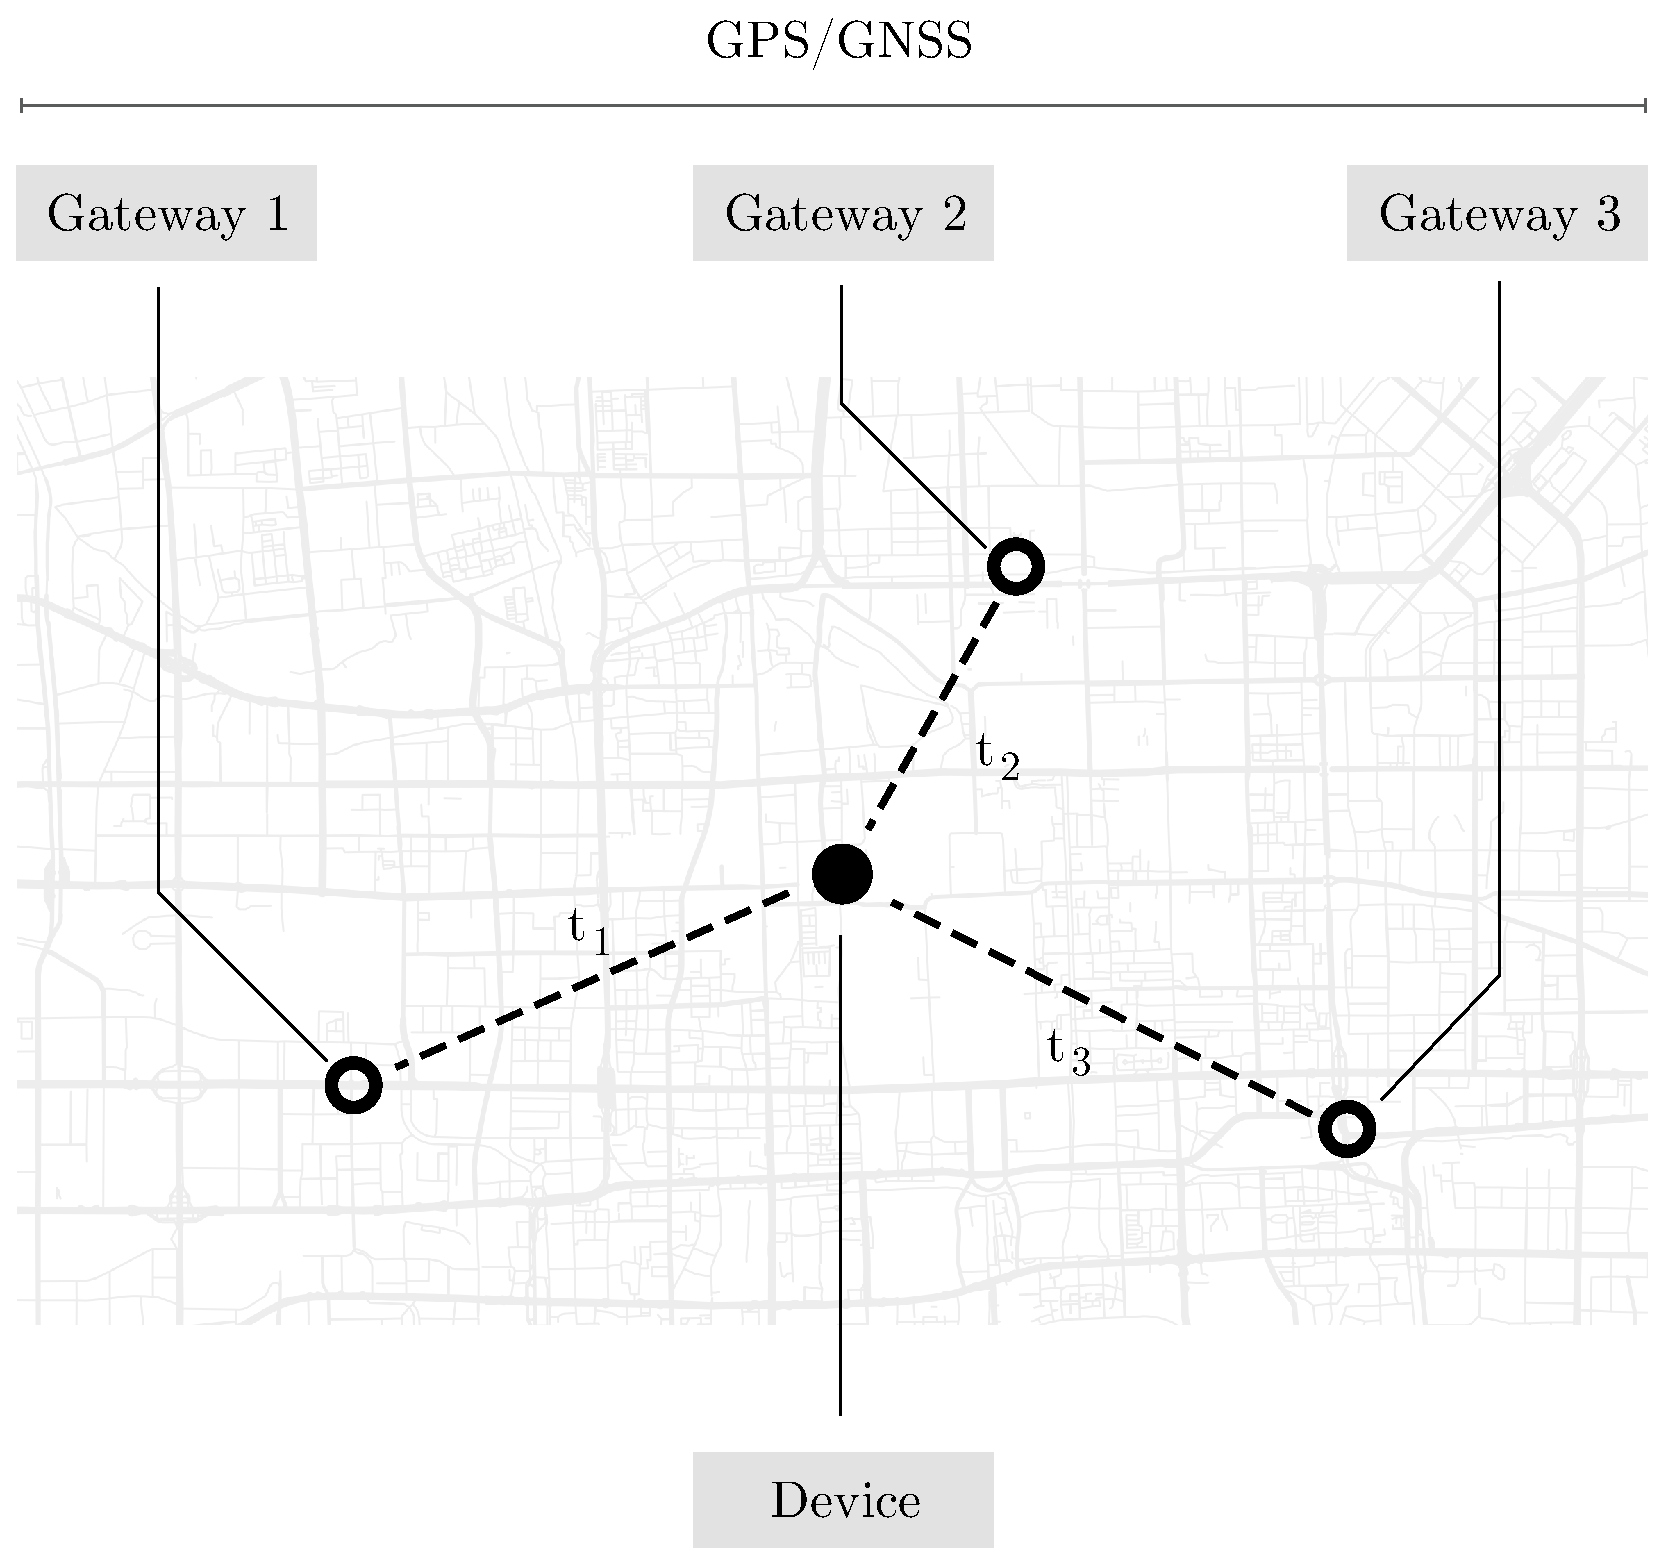
\includegraphics[width=\columnwidth]{tdoa.eps}
          \caption{\emph{Geolocation via TDoA}}
          \label{fig:tdoa}
     \end{center}
\end{figure}

Typically it is challenging to accurately record $T_n$, as any nanosecond-level variance in the timestamp can lead to significant variance in the resulting location solution. To achieve this level of precision it is necessary to use extremely high-bandwidth raw \emph{in-phase and quadrature (I/Q) data} from the miners radio hardware and a fast enough processor to sample this data, identify an appropriate packet, and record the timestamp. Typically a \emph{Field Programmable Gate Arrays (FPGA)} is used as the processor for this data, however these are fairly expensive, power hungry, and emit significant heat. Instead, the reference Helium Gateway mining hardware uses a novel technique using commodity low-cost components to process I/Q data and achieve timestamping at this level of precision. Further information on the techniques, components and schematics used will be released as open source software at network launch.

\textbf{Using timestamps to derive location}. Now that the devices router, $R$, is in posession of a variety of signed messages which include the precise timestamps $T_n$ it is possible to \emph{solve} for the location of the device $D$. A variety of TDoA algorithms exist such as \todo{\cite{}, \cite{} and \cite{}}. We choose to implement the method described by \emph{Kim} and refer the interested reader to \todo{\cite{}} for greater detail on the algorithm and implementation. If a sufficient density of $M_n$ and therefore $T_n$ are recoreded for a given packet, the location of $D$ can be derived down to a few meters depending on a variety of factors.

\textbf{Verifying cryptographic \emph{Proof-of-Location}}. \todo{BLAH BLAH} Because of the expense and power consumption of a typical GPS module, and the fact that they require a view of the sky, providing geolocation as a network service makes devices cheaper, more power efficient, and able to located accurately indoors. Additionally, because these data transmission events occur in the context of a blockchain, unforgeable cryptographic proof of location for a device can be obtained. Devices being able to prove they were in a specific place at a specific time has tremendous potential for a wide variety of machine applications.

\section{Transactions}\label{transactions}

Transactions in the Helium blockchain provide functionality that enables address-to-address transfers of Helium tokens, similar to many existing blockchain networks, but also provide a set of primitives that enable core functionality that is critical to the operation of a \verb|DMN|. In this section we address the philosophy behind our transaction system, the primitives, and the way fees on the network work. We will first address Helium's need for microtransactions and propose a new solution.

\subsection{Microtransactions} \label{microtransactions}

In this section we discuss Helium's need for microtransactions, the limitations of existing solutions, and propose a solution based on staking and burning.

\subsubsection{Helium's Need for Microtransactions}

\paragraph{Devices Pay Per Packet}
The goal of Helium is to provide internet data transport fees (the fees paid by devices to miners) that are an order of magnitude less than anything currently available for this type of service. This transport fee would need to be metered per-packet in order to allow for maximum flexibility --- this way, a device could transact with any miner, even just to send or receive a single packet without having previously established a relationship with that miner.

\paragraph{All Transactions Occur On-Chain}
Helium is built on the philosophy that all transactions should occur \emph{on-chain}; that is, blocks should be sized and mined with a frequency such that every transaction which occurs on the network should be stored in the blockchain.  To accomplish this goal the cost of mining must be low, blocks must be large enough to encapsulate a large number of transactions, and frequent enough that transactions are processed quickly.

\paragraph{Allow Devices to Persist Data to the Blockchain}
Because the Helium blockchain services a specific use, the \verb|DMN|, blocks must additionally be able store fingerprints of data sent from devices along with the transaction which pays a miner for their transport service.  We believe that this holistic \emph{tamper-proof} data trail will enable entirely new use cases where the authenticity and veracity of sensor data is critical.

\subsubsection{Limitations of Existing Solutions}

Now that we have discussed the requirements of transactions within Helium, we outline the existing solutions for micropayments on a blockchain and address their shortcommings as they apply to our network.

\paragraph{Heavyweight Transactions}
This first option is suitable only for larger transactions as the service fee is smaller than the payment. This method does not work well for very small transactions as whoever pays the transaction fee ends up potentially paying more for the transaction fees than the value being exchanged. This is a similar problem to buying small-value items using credit cards today. The vendor pays a minimum fee on each credit card transaction, and under a certain charge they lose money on the transaction. These heavyweight transactions are clearly not suitable for use as a micro transaction system within Helium.

\paragraph{Zero-fee Transactions}
While highly desirable from a device perspective, a true zero-fee blockchain would be frought with spam transactions. It would be trivial to write a script to pollute the blockchain with transactions meant only to waste space on the blockchain and increase congestion on the network. Some ostensibly zero-fee blockchain implementations solve this issue in clever ways, such as offloading the work of processing and verifying transactions to the transactors themselves \cite{iota}. However, these implementations have their own issues, for example IOTA has not yet proved it is capable of operating this type of system without the need for a centralized coordinator.

\paragraph{State Channels}
State channels \cite{state-channels} allow two parties to exchange value, usually in small increments at a time, with very limited risk. If one party thinks the other is acting dishonestly, they can publish the final transaction in the state channel to the blockchain and close the channel. At most one payment is usually at risk. However, there are several downsides: the payer has to lock up significant funds for the lifetime of the state channel, meaning they may be unable to open state channels with other parties or pay other dues; transactions in the state channel do not appear on the main chain at all; and these implementations are relatively complex to execute well (note that neither Lightning \cite{lightning} nor Raiden \cite{raiden} have become widely used yet).

\paragraph{Payment in Arrear}
Payment in arrear, after the services have been rendered, is an extremely risky method in a decentralized pseudo-anonymous system. There is no mechanism to gain certainty around the intent or honesty of the entities transacting, nor do you know if the entities control the requisite funds when the debt comes due. This model only works when the parties involved trust each other, or have some other recourse to recover funds.

\subsubsection{A Proposed Solution Based on Staking \& Chits}

In order to satisfy our requirement of on-blockchain micro transactions with no fees, we propose a system that takes inspiration from staking and state channels.

In order for devices to issue zero fee payments to miners, they must first stake a \emph{deposit} of tokens using the \emph{create\_deposit} transaction \secref{primitives}. This transaction has a fee. Once the initial deposit has been created, the network user can proceed to issue \emph{chits} against their deposit until it is exhaused. Chits are a type of transaction; a promissory note that payment will be delivered in the future, and enough information to trust a favorable outcome. These chits are returned in response to a gateway offering a packet for delivery. Chits are linked to each other; the blockchain needs to have seen the previous chits before subsequent ones will be accepted. Each chit references the deposit, the sequence number (nonce), the amount to pay and any additional information about the packet.

Because the miner concerned wants to be paid for transport, it will add the chit to its mempool, along with any previous chits that it depends on. This means that several miners are all incentivized to include these chits in their current blockchain. The entity issuing \emph{chits} can use the final \emph{chit} in the transaction chain to incentivize a miner to include all the previous (or missing) chits in a block. If previous chits are not included in the chain, nobody gets paid.

At first glance this is similar to how state channels work, but with a couple of significant differences. State channels are a one to one construct, while chits can be one to many. Critically, this method keeps the record of all included transactions on-chain. The crucial benefit to this design is that all transaction fees for these payments can be eliminated. The first staking transaction can be sent along with the first chit, so the gateway is incentivized to add it to their block. If the first miner doesn't include it, the second \emph{chit} can be accompanied with the staking transaction and the first chit when communicating with the next miner. Eventually the advantage of including the transactions outweighs the disadvantages.

It is important to note that nobody gets paid until everybody gets paid. Chits should not be issued after the \emph{ExpiryHeight}. If the deposit is not distributed $n$ blocks after the ExpiryHeight, the deposit is disbursed as much as possible and any remaining balance is destroyed. This provides an incentive for everyone involved to settle the balance.

\subsubsection{Example Deposit Lifecycle}

In this section, we will walk through an example lifecycle of a router staking a deposit, miners performing work on behalf of the router, and being compensated by the router through chits against the deposit. See \secref{cycle:router} for a more detailed set of protocols related to the router deposit and data lifecycle.

\begin{enumerate}

\item A router $R$ creates a deposit $S$ of 500 tokens, expiring at block height $current\_height$ + $\lambda$, by publishing a \verb|create_deposit| transaction and paying a nominal transaction fee
\item A miner $M_1$ hears a packet $P_1$ broadcast by device $D$
\item $M_1$ uses the address of $D$, attached to $P_1$, to identify $R$ as the owner of $D$
\item $M_1$ sends the signature $K(P_1)$ of $P_1$ and an offer of 1 token for transport to $R$
\item $R$ receives $K(P_1)$ and the payment offer and determines if it accepts the packet for the offered price
\item Assuming $R$ accepts the packet at the offered price, it constructs a \textbf{chit} transaction $C_1$ with nonce 1, with a value of 1 token, payable to $M_1$, against $S$ and sends it to $M_1$
\item Having received $C_1$, $M_1$ verifies the correctness of $C_1$ by inspecting $S$ on the blockchain and sends $P$ to $R$
\item $M_1$ adds $C_1$ to its mempool and gossips it to the peer-to-peer internet network
\item Meanwhile, $D$ has physically moved and broadcasts its next packet $P_2$. A different miner $M_2$ now hears $P_2$
\item Just as before, $M_2$ sends $K(P_2)$ to $R$ along with an offer of 0.9 tokens for transport
\item $R$ responds with a chit $C_2$, but since $C_1$ has not been included in a block yet, and chits must be included in nonce order, $R$ also sends $C_1$
\item $M_2$ adds $C_1$ and $C_2$ to its mempool and gossips both chit transactions to the peer-to-peer network
\item $M_1$, being invested in deposit $S$, hears about the new chit $C_2$ over the peer-to-peer network and adds it to its mempool
\item $R$ continues issuing chits $C_n$ against $S$ until either:
  \begin{enumerate}
  \item The value of $S$ is depleted, at which point $R$ can create a new deposit
  \item $S$ expires at the previously specified block height and the remaining balance is burned
  \end{enumerate}
\item Once $S$ is closed either through depletion or expiration, all gateways owning chits against $S$ receive their payment
\end{enumerate}

\subsubsection{Problems \& Solutions}

In this section we address potential problems that could arise with the deposit \& chit approach and present solutions to these problems.

\paragraph{Degenerate Miner} A miner, after being issued a chit for the service it has agreed to perform, could neglect to follow through and perform the service. If a miner fails to send the agreed packet to the router after the router issues a chit, the router can re-request it (for some period of time). The threat of losing future business from a router and the relatively low overhead of completing the transfer of the packet acts to disincentivize miners from acting in bad faith. This is consistent with state channel implementations where the task is subdivided such that the scope of potential loss is below a meaningful threshold.

\paragraph{Chit Bomb} A malicious actor could stake a deposit and then proceed to issue a near limitless amount of miniscule chits against that deposit without incurring transaction fees. This could flood mempools and pollute the blockchain with spam transactions. Assuming we trust our network of miners \secref{scores}, this could never happen. Miners are the only entity on the network capable of creating new blocks for the blockchain, and chits can only be issued to miners in payment for their services. Because we assume all miners to be rational actors, we anticipate they will only include transactions that benefit themselves. These are either transactions with fees attached, or chits that they have a direct investment in, either because they will get paid, or because the transaction is attached to a stake in which they have chits. Therefore, we expect miners to ignore any spam chits that were not issued in exchange for a service provided.

\paragraph{Final Transaction}
In theory, it is possible for the chit issuer to spend all the staked tokens and not have anything left to incentivize a miner to include the final transaction. All the miners involved in the chain of chits have an incentive to get the transaction included in a block, and because there is a fair chance of any individual miner winning a block, this should eventually clear.

\subsection{Light Clients \& Full Nodes} \label{full-nodes}

Until now, we have discussed how to deal with microtransactions in a cost-effective way, however we have not yet addressed how to deal with the inevitable continuously increasing size of the blockchain. One requirement for Helium is that all transactions occur on-chain. This means that the size of the full blockchain will eventually grow quite large. This is compounded by the fact that all miners on the network are gateway devices, relatively limited in computation power and storage space.

We solve this constraint by allowing mining nodes to operate as \emph{light clients} on the blockchain, pruning old blocks and transactions as needed and keeping only the latest ledger values. They will communicate over the peer-to-peer network with \emph{full nodes} which maintain a complete history of the blockchain to verify transactions.

This raises a question: who is responsible for operating full nodes, and what is their incentive to do so? Routers are software-only applications with access to scalable, cloud-based storage and will be required to operate full nodes in order to fulfill their purpose. Helium Systems Inc will operate a set of hosted routers that will make it easy for developers to launch products without needing to deploy their own router. However, many enterprise developers, who are required to maintain a higher standard of privacy, will want to host their own router. Together, these routers will form a network of full nodes capable of supporting resource constrained gateways and wallets operating light clients.

\subsection{Fees} \label{fees}

Transaction fees are an essential part of most blockchain implementations. They incentivize miners to include a transaction in their draft block and ensure that spam transactions do not pollute the blockchain and network. We've discussed how the \emph{chit} transaction \secref{chit} is able to eliminate fees in the prior section on Microtransactions \secref{microtransactions}. However, all other transactions on the \verb|DMN| require transaction fees.

To determine the appropriate fee for a new transaction, the transactor will take the median of the past $\delta$ packet transport fees, within some margin of error. Until $\delta$ packet transports have been completed, the fee will be fixed at a constant value $\alpha$. By anchoring the transaction fee to the current fees being charged for transport on the network, we root them in reality. Helium's primary purpose is to facilitate a network of wireless ineternet coverage. In order to accomplish this in the long term, all of the economics of the system must align to make it practical for the primary users to transact on the network. If one set of fees were to outstrip the other, the network would quickly lose its utility for the key user segment.

To enable miners and other light clients to determine an appropriate fee, full nodes \secref{full-nodes} will expose a fee suggestion API. This way resource constrained entities that do not maintain a complete copy of the blockchain will not need to compute the fee from the most recent transactions. When submitting a block, peer miners will verify the correctness of the block and ensure that no fee has deviated beyond the acceptable threshold of $\delta$.

\subsection{Staking} \label{staking}

The \emph{assert\_location} transaction, mentioned below \secref{primitives}, has a special type of fee calculation; a \emph{dynamic} fee. Because the Helium network reaches maximum \emph{usefulness} at a specific density of gateways, we want the fees to incentivize the network density to be as close to that ideal as possible. To that end, the transaction fee for asserting a location can be thought of as the y coordinate on a curve with the formula \[\mathit{y = \left(x - D\right)^4 + F}\] where $D$ is the ideal gateway density and $F$ is the unit fee for a location transaction. A sample graph of this function where $D$ = 3 and $F$ = 1 follows:

\pgfplotsset{width=12cm,compat=1.9}
\begin{tikzpicture}[scale=\columnwidth/12cm]
    \begin{axis}[xlabel = Density, ylabel = Fee]
        \addplot[color=gray, domain=0:6]{(x - 3)^4 + 1};
    \end{axis}
\end{tikzpicture}

As can be seen, gateways near the ideal network density are cheap to add, but establishing a new network or overpopulating a network gets expensive very quickly. This serves to dis-incentivize gateway deployments that are not beneficial to the network. In particular, \emph{Alternate Reality Attacks} and warehouses full of miners become prohibitively expensive.

Blocks submitted to the network by miners who have not asserted their location, and therefore not paid the staking fee, will be considered invalid and not considered by miners for inclusion in the chain.

Miners who move physical location will need to assert a new location, and pay the new staking fee.

\subsection{Primitives in Helium} \label{primitives}
Having discussed the philosophy of our transaction system and presented our approach to facilitating zero-fee mictrotransactions on the Helium network, we now delineate the transaction primitives and their properties.

\begin{description}
  \item [add\_gateway] Registers a new gateway on the network, adding it to an existing account which will be responsible for supplying its stake (required for mining) and will receive mining rewards \secref{mining} and fees earned by the gateway

\begin{table}[H]
  \centering
  \begin{tabularx}{\columnwidth}{l X}
    \toprule
    Property & Description \\ \midrule
    gateway\_address & the address of the gateway being added to the network \\
    public\_key & the public key of the gateway being added to the network \\
    owner\_address & the address of the owner account \\
    signatures & mutual signatures of the owner and gateway
  \end{tabularx}
\end{table}

\item [assert\_location] Asserts a gateway's location in the form of geographic coordinates, requiring a dynamic stake

\begin{table}[H]
  \centering
  \begin{tabularx}{\columnwidth}{l X}
      \toprule
      Property & Description \\ \midrule
      gateway\_address & the address asserting its location \\
      nonce & a monotoically increasing integer \\
      latitude & the latitude of the gateway \\
      longitude & the longitude of the gateway \\
      altitude & the altitude of the gateway \\
      signature & the signature of the gateway
  \end{tabularx}
\end{table}

\item [payment] \label{payment} Moves tokens from one account, the \emph{payer}, to another account, the \emph{payee}. N.B. this payment transaction requires a fee, while \emph{chit} \secref{chit} does not.

\begin{table}[H]
  \centering
  \begin{tabularx}{\columnwidth}{l X}
      \toprule
      Property & Description \\ \midrule
      payer\_address & the address of the sender \\
      payee\_address & the address of the recipient \\
      nonce & a monotoically increasing integer \\
      value & an integer-based representation of the tokens to send \\
      signature & the signature of the sender
  \end{tabularx}
\end{table}

\item [create\_deposit] Creates a staked deposit which can later be fractionally issued and redeemed in the form of \emph{chits} \secref{chit} without incurring transaction fees. Any unused portion of the deposit will be burned after some time.

\begin{table}[H]
  \centering
  \begin{tabularx}{\columnwidth}{l X}
      \toprule
      Property & Description \\ \midrule
      address & the address of the account creating the deposit \\
      value & an integer-based representation of the deposit amount \\
      public\_key & an ephemeral public key used for signing chits for this deposit \\
      expiry\_height & the block height at which this stake expires \\
      signature & the signature of the depositor
  \end{tabularx}
\end{table}

\item [chit] \label{chit} Issues a chit against a previously staked deposit in payment for transport or other services. N.B. this payment transaction does not require a fee, while \emph{payment} \secref{payment} does.

\begin{table}[H]
  \centering
  \begin{tabularx}{\columnwidth}{l X}
      \toprule
      Property & Description \\ \midrule
      public\_key & the public key used to create the deposit \\
      value & an integer-based representaion of the value of the chit \\
      nonce & a monotoically increasing integer \\
      packet\_reference & a hash of the packet being paid for \\
      payee\_address & the address of the recipient \\
      signature & the signature of the depositor
  \end{tabularx}
\end{table}

\end{description}

\section{Helium Consensus Protocol}\label{consensus}

Instead of an extremely computationally expensive and power hungry \emph{Proof-of-Work}, Helium miners generate \emph{Proofs-of-Coverage} \secref{poc}. In this section we present how these useful proofs can be used to create permisionless network consensus.

\subsection{Motivation}

Many current generation blockchains rely on a computationally difficult \emph{Proof-of-Work} to protect the network against sybil attacks, also known as \emph{Nakamoto Consensus}. The fact that the \emph{Proof-of-Work} is computationally expensive to create, but cheap to verify means that in order to propose a new valid block to the network there is evidence that a significant amount of computation has been expended. Due to the fact that computation is limited by hardware cost, power cost, physical space and computational efficiency of modern technology, sybil attacks become impossible. However, this approach, while fundamental to the mainstream adoption of blockchain technology, has several downsides. Chief among the downsides is the power consumption; it is estimated that the Bitcoin network is consuming more power than many small countries. Bitcoin's PoW is so wasteful it is now on the list of the top uses of electricity in the world and whenever the value of Bitcoin goes up, so do the resources devoted to mining it.

Related to the power problem is the mining pool problem. Many blockchains have mining pools where users band together to, in parallel, mine a single block; listing the pool's address as the party to get paid. The pool then shares the block reward with the members of the pool. This ends up defeating many of the advantages of decentralization as both Bitcoin and Ethereum have come to be dominated by less than 10 mining pools each. These large pools effectively prevent independent parties from mining blocks on their own. This means that the consensus protocol for these blockchains is effectively controlled by a very small number of mining pools and risks becoming further centralized.

More recently there has been increased momentum around making blockchain consensus protocols less wasteful and more useful to the network. Filecoin \cite{filecoin} has a \emph{Proof-of-Spacetime} and Ethereum \cite{ethereum} is moving towards a \emph{Proof-of-Stake} \cite{pos} approach.

For Helium, we desire a consensus protocol with the following attributes:

\begin{itemize}
  \item \textbf{Permisionless}: nodes should be able to freely participate in the network without permission or approval from any other entity, as long as those nodes operate in accordance with the consensus rules.
  \item \textbf{Extremely decentralized in nature}: network consensus should be designed such that there is no incentive available for taking advantage of macro-economic factors, such as cheaper access to electricity in certain geographies, and that simply buying more hardware in the same location is either ineffective or cost prohibitive. Additionally, it should be impossible for mining pools to form and for groups to collaborate in mining blocks.
  \item \textbf{Byzantine Fault Tolerant}: the protocol should be tolerant of Byzantine failures \cite{byzantine-failures} such that consensus can still be reached as long as a majority of actors are acting honestly. 
  \item \textbf{Based on useful work}: achieving network consensus should be \emph{useful} and \emph{reusable} to the network. Work performed in Nakamoto Consensus-based systems is only useful for the particular block being mined and is not otherwise useful or resuable on the network. An ideal consensus system would contain work which is both useful and reusable to the network beyond simply securing the blockchain.
  \item \textbf{High confirmed transaction rate}: our ideal consensus protocol would be able to process a very high number of transactions per second, and once a transaction is seen in a block it would be considered confirmed. Many existing blockchains require a lengthy \emph{settlement time} while the network achieves consensus which is not ideal in a system like Helium which may experience a very high number of transactions and where waiting for a transaction to settle is not tenable.
  \item \textbf{Transactions are censor-resistant}: ideally miners would not be able to censor or otherwise pick and choose transactions prior to mining them. This would not only nullify any attempts to nefariously censor transactions, but would allow for otherwise unattractive transactions (such as fixed-fee transactions) to be included in the blockchain.
\end{itemize}

The remainder of this section lays out our construction of a consensus protocol with these design goals in mind that we refer to as the \emph{Helium Consensus Protocol (HCP)}.

\subsection{HCP}

We propose a unique consensus protocol around \emph{Proof-of-Coverage} to capture the useful work of verifying the network as a replacement for \emph{Proof-of-Work}, combined with a variant of the \emph{HoneyBadgerBFT (HBFT)} \cite{honeybadger} asynchronous byzantine fault tolerant protocol.

\textbf{HBFT}. HBFT is an asynchronous atomic broadcast protocol to achieve optimal asymptotic efficiency, initially presented by Miller et al in 2016. In HBFT, the setting assumes a network of $N$ designated nodes with distinct well-known identities ($P_0$ through $P$\textsubscript{N−1}). In our HCP instantiation this network of nodes is known as the consensus group $C$. The consensus group receive transactions as input, and their goal is to reach common agreement on an ordering of these transactions and form them in to blocks to be added to the blockchain.

The protocol proceeds in epochs, where after each epoch, a new batch of transactions is appended to the blockchain. At the beginning of each epoch, the group choose a subset of the transactions in their buffer, and provide them as input to an instance of a randomized agreement protocol. At the end of the agreement protocol, the final set of transactions for this epoch is chosen.

HBFT relies on a \emph{threshold encryption} scheme that requires transactions be encrypted to a master public key, such that the consensus group must work together to decrypt it. This means that no individual node is able to decrypt or censor a particular transaction without colluding with the majority of the group. 

\textbf{Applying \emph{Proof-of-Coverage} to HBFT}. In Helium, miners are required to submit \emph{Proofs-of-Coverage} to the network at an epoch $\Delta_p$. These proofs are submitted as a special type of transaction, and subsequently recorded to the blockchain. As detailed in \secref{poc}, Helium miners increase their \emph{score} as they submit valid proofs to the network. At an epoch $\Delta_c$ the highest scoring miners, $N$, are elected as the new HBFT consensus group $C$.

By using \emph{Proof-of-Coverage} to elect the members of $C$ we are essentially substituting for well-known identities in the HBFT protocol. As we desire a \emph{permisionless} network, we can use \emph{Proofs-of-Coverage} to determine whether miners are acting honestly and reward the \emph{most honest} miners at a given epoch by electing them to the HBFT consensus group.

\textbf{The consensus group}. Once the consensus group $C$ has been elected for a given $\Delta_c$ epoch, a key generation phase occurs using a threshold encryption scheme \verb|TPKE|. \verb|TPKE| is a cryptographic primitive that allows any party to encrypt a transaction to a master public key \verb|PK|, such that $C$ must work together to decrypt it. Once $f + 1$\footnote{$f$ is a protocol parameter equal to the number of tolerable byzantine faults} correct members of $C$ compute and reveal decryption shares, $\sigma_i$, the transaction can be recovered. Once \verb|PK| is generated via the \verb|TPKE.Setup| function, a block containing \verb|PK| is immediately submitted to the blockchain. Each member $N_m$ in $C$ receives a \emph{secret key share}, \verb|SK|\textsubscript{i}, of \verb|PK|. 

New blocks are created by $C$ at a fixed interval $\Delta_b$ and recorded to the blockchain. A token block reward is split among the members of $C$ for every block submitted, along with the sum of all fees contained within valid transactions. 

Miners on the network encrypt new transactions $t$ using the \verb|TPKE.Enc(PK|, $t$) $\rightarrow e$ function and submit them to $C$ to be included in the next block. As members of $C$ receive $e$ they run the \verb|TPKE.DecShare(SK|\textsubscript{i}, $e$) $\rightarrow \sigma_i$ function to produce their decryption share. Members broadcast their $\sigma_i$ to the other members of $C$, and once $f + 1$ members have seen $\sigma_i$ shares they can proceed to the \verb|TPKE.Dec| function using \verb|PK|, $e$ and the $\sigma_i$ shares and attempt to decrypt the transaction. Each member of $C$ appends decrypted transactions to their own instantiation of the next block kept in a local buffer. Double-spend and other malformed transactions are removed from these blocks based on the consensus protocol.

As members of the group cannot decrypt transactions on their own, it is not possible for a transaction to be censored by a given member prior to its inclusion in their block without $f + 1$ members of $C$ colluding as transactions are received. As the members of $C$ for a $\Delta_c$ epoch are selected based on their submitted \emph{Proofs-of-Coverage}, making the members anonymous, this type of collusion would be extremely challenging to execute.

Once $\Delta_b$ has elapsed, all members of $C$ run the \verb|TPKE.Enc| function on their locally stored block and broadcast the resulting ciphertext to the other members of $C$. Again, the members run \verb|TPKE.DecShare| on the ciphertext of the block, broadcast their decryption share, and once $f + 1$ have been seen, \verb|TPKE.Dec| is run on the block and it is added to the blockchain. If no consensus can be reached on a valid block by $\Delta_b$, an empty block is appended to the blockchain.

\textbf{Conclusion}. We have presented our consensus protocol which combines a modern, asynchronous and highly efficient Byzantine Fault Tolerant consensus protocol with a novel mechanism for substituting permissioned identity with a useful and reusable \emph{Proof-of-Coverage}. The resultant protocol satisfies the design requirements of being permisionless, decentralized, byzantine fault tolerant, based on useful work, with a very high-rate censor proof transaction mechanism.

We refer the interested reader to \cite{honeybadger} for a detailed breakdown and analysis of the HoneyBadgerBFT protocol.

\section{Network Protocol}

In this section, we provide a more formal overview of the Helium \verb|DMN| and the functions that Devices, Miners, and Routers play in the system.

\subsubsection{Device Cycle}

We provide a brief overview of the device cycle and the functions available to devices on the network in \protoref{proto:device}

\begin{protocol}{Device Protocol Overview}{proto:device}
  \SetKwProg{Device}{\BlankLine Device}{}{}

  \Device{at any time} {
    Send data \;
    Receive data \;
  }

  \Device{when provisioning} {
    Generate keypair \;
    Input configuration information \;
    Store key material \;
    Output public key material \;
  }
\end{protocol}


\begin{description}
  \item [Provisioning] A device is provisioned on the \verb|DMN|.

    Devices join the network with keying material programmed by their owner. This keying material includes a private key known only by the device, the public key of the root-of-trust for the organization and a 64-bit MAC address.The MAC address consists of 32 bits of an Organizationally Unique Identifier (OUI) and 32 bits of an organizationally managed device identifier. Via an out of band mechanism, the device's public key is added to the organization's device registry, indexed by the MAC address. Details of the management of device identifiers and keys are implementation-defined, and out of the scope of this document.

    \begin{protocol}{Device Provisioning}{proto:device.provision}
      \SetKwProg{Prov}{\BlankLine Provision}{}{}
      \SetKwFunction{Store}{Store}
      \SetKwFunction{Encrypt}{Encrypt}

      \Prov{device D} {
        $E_k, E_{pk}, \leftarrow $ generate public/private keypair \;
        Input ${ID}_d \leftarrow $ $ \ll device ID:32 \gg $ \;
        Input $R_k \leftarrow $ public key for organization \;
        Input ${OUI}_d \leftarrow $ $ \ll organization ID:32 \gg $ \;
        \BlankLine
        Securely \Store{$E_k$, $E_{pk}$, $R_k$, ${OUI}_d$, ${ID}_d$} \;
        \BlankLine
        Output $E_k$ \;
      }
    \end{protocol}


  \item [Send] A device sends data to a router on the internet, via a miner.

    Devices can send data to their specified router on the internet by paying miners Helium tokens.
    A device initiates the sending process by broadcasting a packet via the wireless protocol. When a device broadcasts a packet, any miners in a reasonable geographic area hear it. Each packet header contains the device's MAC address, and miners inspect the blockchain using this address to determine which routers are listed for the OUI component of the MAC address. See the Miner Deliver \protoref{proto:miner.data.deliver}.

    \begin{protocol}{Device Send Data}{proto:device.data.send}
      \SetKwProg{Recv}{\BlankLine Receive}{}{}
      \SetKwProg{Send}{\BlankLine Send}{}{}
      \SetKwFunction{SignalData}{SignalData}
      \SetKwFunction{Data}{Data}
      \SetKwFunction{Transmit}{Transmit}

      \Send{from device ${ID}_d$, packet P} {
        $M \leftarrow $ \SignalData{P} \;
        \Transmit{M} \;
        \BlankLine

        $P_e \leftarrow $ \Encrypt{P, private key $E_{pk}$} \;
        $B \leftarrow $ \Data{${OUI}_d$, ${ID}_d$, $P_e$} \;
        \Transmit{B} \;
        \BlankLine

        \Switch{Wait for response} {
          \Case{signaling message M} {
            Recieve Data. See \protoref{proto:device.data.recv}
          }
          \Case{timeout} {sleep}
        }
      }
    \end{protocol}


  \item [Receive] After a device performs a Send, it listens for a response.

    The response can be a single acknowledgment or a queued up command or data packet. If the device gets a signaling packet describing a downlink message, it stays awake until the entire packet is received, otherwise, it is free to turn its radio off or go into power-saving mode.

    \begin{protocol}{Device Receive Data}{proto:device.data.recv}
      \SetKwProg{Recv}{\BlankLine Receive}{}{}
      \SetKwFunction{Decode}{Decode}

      \Recv{at device ${ID}_d$, signaling message M} {
        Size $S \leftarrow $ \Decode{M} \;
        \Switch{Receive Packet P} {
          \Case{success} {hand to application}
          \Case{timeout} {sleep}
        }
      }
    \end{protocol}


\end{description}


\subsubsection{Miner Cycle}\label{mining}

We provide a brief overview of the mining cycle and the functions available to miners on the network in \protoref{proto:miner}.

\begin{protocol}{Miner Protocol Overview}{proto:miner}
  \SetKwProg{Miner}{\BlankLine Miner}{}{}

  \Miner{at every epoch \emph{blocktime}} {
    Construct a block\;
    Add transactions from non-winning blocks\;
    Add transactions from mempool\;
    Construct \emph{Proof-of-Coverage}\;
    Construct \emph{Proof-of-Serialization}\;
    Submit block to peers\;
  }

  \Miner{at any time} {
    Receive transactions\;
    Receive block\;
    Receive PoC challenge\;
    Receive radio challenge\;
    Receive serialization challenge\;
    Receive data from device\;
    Receive data from router\;
  }

  \Miner{when joining} {
    Construct transaction with address, public key, and payee\;
    Construct transaction with location\;
    Submit transactions to a random peer\;
  }

  \Miner{on location change} {
    Construct transaction with new location\;
    Submit transaction to a ramdom peer\;
  }
\end{protocol}



\begin{description}
  \item [Join] A miner joins the network.

    Joining the network is merely adding the miner's address/public key and its 'owner' (the address mining rewards should be paid to) to the blockchain.

  \item [Assert Location] A miner asserts their GPS location to the network.

    Asserting a location indicates that the miner is claiming it is at particular physical coordinates. To assert a location, a dynamic stake is required. The value of the dynamic stake is related to a parabolic curve where the x-axis represents the density of the existing network in that area, and the y-axis is the staking multiplier. Thus for singleton gateways or small networks, the staking requirements are high.  Once the network approaches an ideal density, the stake approaches the minimum. Then, as the density of the network exceeds the ideal, staking costs increase. This final increase disincentivizes \emph{Alternate Reality Attacks} because asserting a location in an unpopulated region with no way to confirm network presence is very expensive. Similarly, constructing a `mining warehouse' with an extremely high density of miners becomes prohibitively expensive. Only miners that have asserted a location are allowed to mine. Assertions of location can be retracted and the stake recovered, or they can be confiscated in cases of misbehavior.

  \item [Receive Transactions] A miner connects to the peer-to-peer network and listens for clients publishing transactions to the network.

    Transactions contain fees that the miner can claim if it publishes the winning block \secref{fees}. The miner can also capture transactions from blocks published to the peer-to-peer network that did not win as described in \protoref{proto:miner.block.recv}.


    \begin{protocol}{Miner Receive Transactions}{proto:miner.trans.recv}
      \SetKwProg{Recv}{\BlankLine Receive}{}{}

      \Recv{transactions} {
        Add transactions to mempool\;
      }
    \end{protocol}


  \item [Construct Block] The miner takes the current head of the chain and begins to construct a new block.

    The new block contains the hash of the previous block (the current head), the block height (how many blocks are in the chain between this block and the genesis block) and a set of transactions from the mempool. The set of transactions are added to a Merkle tree, and the root hash is also stored.

  \item [Construct PoC] A miner begins the \emph{Proof-of-Coverage} process by becoming a Challenger.

    The miner uses their public key to sign a digest of their partially completed block to obtain some verifiable randomness. This randomness is used to choose the Target. Once the Target is selected the proof of coverage is constructed and deliver to the Target to begin the challenge as detailed in \secref{poc}.


    \begin{protocol}{Miner PoC Challenge}{proto:miner.poc.challenge}
      \SetKwProg{Challenge}{\BlankLine PoC Challenge}{}{}
      \SetKwFunction{SelectTarget}{SelectTarget}
      \SetKwFunction{SelectCandidates}{SelectCandidates}
      \SetKwFunction{WeightedGraph}{WeightedGraph}
      \SetKwFunction{ShortestPath}{ShortestPath}
      \SetKwFunction{FoldR}{FoldR}
      \SetKwFunction{Encrypt}{Encrypt}
      \SetKwProg{MakeLayer}{\BlankLine MakeLayer}{}{}
      \SetKwFunction{ML}{MakeLayer}

      \Challenge{at challenger C} {
        $T \leftarrow $ \SelectTarget{C}\;
        $T_n \leftarrow $ \SelectCandidates{T}\;
        $T_g \leftarrow $ \WeightedGraph{$T_n$}\;
        $T_{1 \dots l} \leftarrow $ \ShortestPath{$T_g$}\;

        $S \leftarrow $ generate secret \;
        $O \leftarrow $ \FoldR{\MakeLayer{S}, [], $T_{1 \dots l}$} \;
      }

      \MakeLayer{Secret S, [$T_h$ $\vert$ $T_t$]} {
        $E_h \leftarrow $ public key of $T_h$\;

        \Switch{$T_t$} {
          \lCase{[]} { $ \ll \gg $}
          \Other{
            Remainder $R \leftarrow $ \ML{S, $T_t$} \;
            $L \leftarrow $  $\ll S:64, \psi:32, R \gg $ \;
            \Encrypt{L, $E_x$} \;
          }
        }
      }
    \end{protocol}



  \item [Receive PoC Challenge] A miner receives a PoC challenge from one of it's peers.

    A PoC challenge is handed to the first of the targets in the challenge. The target is responsible for immediately transmitting the challenge as described in \secref{poc}.

    \begin{protocol}{Miner PoC Challenge Transmit}{proto:miner.recv.poc.challenge}
      \SetKwProg{Recv}{\BlankLine Receive}{}{}
      \SetKwFunction{Transmit}{Transmit}

      \Recv{at miner T, challenge O} {
        \Transmit{O}\;
      }
    \end{protocol}



  \item [Receive Radio Challenge] A miner receives a \emph{Proof-of-Coverage} radio transmission.

    The miner receives a radio challenge. The challenge contains the original challenger and encrypted data. The encrypted data includes a secret, the next block of data, and the time at which to transmit that remaining data.

    The miner delivers a signed receipt of the secret, next transmission time, and the perceived signal strength to the challenger. Finally, it transmits the next data block at the indicated time to complete the challenge.

    \begin{protocol}{Miner Receive Radio Challenge}{proto:miner.recv.challenge.radio}
      \SetKwProg{Recv}{\BlankLine Receive}{}{}
      \SetKwFunction{Decrypt}{Decrypt}
      \SetKwFunction{Deliver}{Deliver}
      \SetKwFunction{Transmit}{Transmit}
      \SetKwFunction{Sign}{Sign}

      \Recv{radio challenge envelope (challenger C, data O), at time $\beta$, signal strength $\upsilon$} {
        \Switch{\Decrypt(O, private key $E_{pk}$)} {
          \Case{Secret $S$, NextTime $\psi$, Remainder $R$} {
            $K_s \leftarrow \ll S:64, \beta:32, \upsilon:32 \gg $\;
            $B \leftarrow \Sign{$K_s$, $E_{pk}$} $\;
            \Deliver{C, B}\;
            At time $\psi$ \Transmit{(C, R)}\;
          }
          \lOther{drop challenge}
        }
      }
    \end{protocol}


  \item [Receive Serialization Challenge] A miner receives serialization challenges from other miners trying to construct a proof.

    The miner returns a signed envelope including the challenge and the current time. The challenging miner uses a number of these serialization challenges to prove that the final \emph{Proof-of-Coverage} happened at a given time.

    \begin{protocol}{Miner Receive Serialization Challenge}{proto:miner.recv.challenge.serialization}
      \SetKwProg{Recv}{\BlankLine Receive}{}{}
      \SetKwFunction{Time}{Time}
      \SetKwFunction{Sign}{Sign}

      \Recv{serialization challenge K}{
        $T \leftarrow \Time{milliseconds} $\;
        $B \leftarrow \ll K:64, T:64 \gg $\;
        $R \leftarrow \Sign{B, $E_{pk}$} $\;
        Respond $R$ to sender\;
      }
    \end{protocol}


  \item [Deliver] A miner delivers data from a device to a router on the internet.

    Once a miner has received a packet from an end device, along with the precise timestamp it was received, it looks up the routers for the organization owning that device and offers the packet to one of those routers, for a fee. The router can accept the fee and return a \emph{chit}, or make a counteroffer. The router can also reject the offer if it already has a copy of the packet or it is unwilling to pay the offered price. A router may pay for several copies of the packet if it wishes to solve for the position of the end device. See the corresponding Router Receive Data \protoref{proto:router.offer.recv}.

    \begin{protocol}{Miner Deliver Device Data}{proto:miner.data.deliver}
      \SetKwProg{Recv}{\BlankLine Receive}{}{}
      \SetKwFunction{FindRouters}{FindRouters}
      \SetKwFunction{CalculateFee}{CalculateFee}
      \SetKwFunction{Sign}{Sign}
      \SetKwFunction{Deliver}{Deliver}
      \SetKwFunction{Hash}{Hash}
      \SetKwFunction{Transaction}{Transaction}
      \SetKwFunction{AcceptableOffer}{AcceptableOffer}

      \Recv{at miner M, timestamp T, from device D, Packet P, Signature $K_p$} {
        Router $R \leftarrow R \in $ \FindRouters{D} \;
        Fee $F_p \leftarrow $ \CalculateFee{R, D, P} \;
        Hash $H_p \leftarrow $ \Hash{P} \;
        Offer $O_p \leftarrow $ \Sign{$\ll ID_d, H_p, K_p, F_p \gg $, $E_{pk}$} \;
        \Switch{\Deliver{R, $O_p$}} {
          \Case{Chit $C_p$}{
            Validate $C_p$\;
            \Deliver{R, T, P}\;
            Submit $C_p$ to peers\;
            Add $C_p$ to mempool\;
          }
          \Case{counter offer ${O\prime}_p$, fee ${F\prime}_p$} {
            Validate ${O\prime}_p$\;
            \Switch{\AcceptableOffer{${O\prime}_p$}} {
              \Case{accept} {
                Restart offer with fee ${F\prime}_p$\;
              }
              \lCase{decline} {
                drop A
              }
            }
          }
          \lOther{drop A}
        }
      }
    \end{protocol}



  \item [Receive Data] A miner receives data from a router on the internet for delivery to a device.

    In response to an uplink packet offer, the router can also respond with a downlink packet, with an attached \emph{chit} to have the gateway deliver a downlink packet to the end device. The end device listens for a downlink packet after transmitting.

    \begin{protocol}{Miner Receive Router Data}{proto:miner.data.receive}
      \SetKwProg{Recv}{\BlankLine Receive}{}{}
      \SetKwFunction{Transmit}{Transmit}
      \SetKwFunction{Transaction}{Transaction}

      \Recv{at miner M, Packet P, signature $K_p$, for device $ID_d$, chit $C_p$} {
        \emph{This can only happen in response to G delivering data to R}
        Validate data $P$ \;
        Validate chit $C_p$\;
        \Transmit{$ID_d$, $ \ll P, K_p \gg $ } \;
        Add $C_p$ to mempool\;
        Submit $C_p$ to peers\;
      }
    \end{protocol}



  \item [Submit Block] A miner submits a new candidate block to the network containing a \emph{Proof-of-Coverage}.

    Once a miner has completed a block, it publishes it to its p2p peers.

    \begin{protocol}{Miner Block Submit}{proto:miner.block.submit}
      \SetKwProg{Submit}{\BlankLine Submit}{}{}

      \Submit{block} {
        Gossip block to peers\;
      }
    \end{protocol}


  \item [Receive Block] A miner receives blocks from one or more of its peers.

    If the received block is considered valid and has not seen it before, the miner gossips it to its peers. Blocks are ranked by their quality: how valuable the proof-of-coverage was, how many transactions were in the block, how many uncles were included, and how close to the ideal blocktime was the time difference from the previous block. After a settling period, each miner chooses its preferred 'best' block and mines the next block on top of that.

    \begin{protocol}{Miner Block Receive}{proto:miner.block.recv}
      \SetKwProg{Recv}{\BlankLine Receive}{}{}

      \Recv{block} {
        Add sender to peer list\;
        Verify block\;
        \Switch{Add block to chain}{
          \Case{success}{
            Gossip block to peers\;
            Harvest losing block transactions\;
          }
          \Case{unchanged}{
            ignore block\;
          }
        }
      }
    \end{protocol}


\end{description}


\subsubsection{Routing Cycle}\label{cycle:router}

We provide a brief overview of the routing cycle and the functions available to routers on the network in \protoref{proto:router}.

\begin{protocol}{Router Protocol Overview}{proto:router}
  \SetKwProg{Router}{\BlankLine Router}{}{}

  \Router{at any time} {
    Create Deposit
    Receive Data Offer \;
    Receive Data \;
  }

  \Router{after receving} {
    Send Device Data \;
  }
\end{protocol}



\begin{description}

\item [Create Deposit] A router creates a deposit to send and receive data packets.

  As described in \secref{transactions} a router makes a deposit in order to declare it is able to receive and send data packets from devices through miners. The deposit is used to issue \emph{chits} when miners offer to deliver packets or when the router needs to deliver data to a device.

    \begin{protocol}{Router Create Deposit}{proto:router.deposit}
      \SetKwProg{Deposit}{\BlankLine Deposit}{}{}
      \SetKwFunction{Transaction}{Transaction}
      \SetKwFunction{Sign}{Sign}

      \Deposit{Amount S, Expiry Height H} {
        Chit Keys $C_k, C_{pk}, \leftarrow $ generate public/private keypair \;
        Transaction $T \leftarrow $ \Transaction(deposit, S, ExpiryHeight, $C_k$) \;
        Add $T$ to mempool\;
        Submit $T$ to peers\;
      }
    \end{protocol}



  \item [Receive Data Offer] A router receives an offer to deliver a device packet.

    This offer includes the address of the device, the hash of the payload, the device's signature of the packet and the proposed delivery fee as described in \protoref{proto:miner.data.deliver}. The router can determine the authenticity of the packet, know if it already has a copy of the packet, and decide on if the delivery price is acceptable.

    A router can accept the offer, decline it or make a counteroffer to the miner. When accepting an offer, the router replies with a \emph{chit} that serves as payment as well as anchoring proof of the packet's existence at that point in time.

    \begin{protocol}{Router Receive Data Offer}{proto:router.offer.recv}
      \SetKwProg{Recv}{\BlankLine Receive}{}{}
      \SetKwFunction{AcceptableOffer}{AcceptableOffer}
      \SetKwFunction{Sign}{Sign}

      \Recv{from miner M, device $ID_d$, packet signature $K_p$, hash $H_p$, fee $F_p$} {
        Verify device $ID_d$ \;
        \Switch{\AcceptableOffer{$F_p$, $ID_d$, $K_p$, $H_p$}}{
          \Case{counter ${F\prime}_c$} {
            Offer $O\prime \leftarrow $ \Sign{$\ll ID_d, H_p, K_p, {F\prime}_c \gg $, $E_{pk}$} \;
            \Deliver{M, $O\prime$}
          }
          \Case{accept} {
            Chit $C \leftarrow $ \Sign{$ \ll accept, ID_d, K_p, F \gg $, $E_{pk}$} \;
            \Deliver{M, C} \;
          }
          \Case{decline} {
            Decline $D \leftarrow $ \Sign{$ \ll decline, ID_d, K_p, F \gg $, $E_{pk}$} \;
            \Deliver{M, D} \;
          }
        }
      }
    \end{protocol}



    \item [Receive Data] A router receives a device packet.

      Once an offer from a miner is accepted, it sends the device packet to the router. The router may accept the same packet multiple times from different miners to perform geo-location on the device.

    \begin{protocol}{Router Receive Data }{proto:router.data.recv}
      \SetKwProg{Recv}{\BlankLine Receive}{}{}

      \Recv{from miner M, device $ID_d$, packet signature $K_p$, packet P} {
        Verify packet $P$ \;
        Process packet \;
      }
    \end{protocol}



    \item [Send Data] On receipt of an offer or data a router can send data to the device.

      Regardless of the accept/decline of the actual packet, the router can leverage the fact that it knows the gateway is in-range of the end-device to send a message down to it. Along with the packet to send, the router includes a \emph{chit} to pay for the transmission.

    \begin{protocol}{Router Send Data }{proto:router.data.send}
      \SetKwProg{Send}{\BlankLine Send}{}{}
      \SetKwFunction{Sign}{Sign}
      \SetKwFunction{Hash}{Hash}
      \SetKwFunction{CalculateFee}{CalculateFee}
      \SetKwFunction{Deliver}{Deliver}

      \Send{using miner M, for device $ID_d$, packet P} {
        $K_p \leftarrow $ \Sign{A, $E_{pk}$} \;
        $H_p \leftarrow $ \Hash(P) \;
        Fee $F_p \leftarrow $ \CalculateFee{$ID_d$, P} \;
        Chit $C \leftarrow $ \Sign{$ \ll deliver, ID_d, K_p, F \gg $, $E_{pk}$} \;
        \Deliver{M, $ID_d$, P, $K_p$, C} \;
      }
    \end{protocol}


\end{description}

\section{Future Work}

This paper presents a well thought-out design for building the Helium network. However, we consider this to be just the beginning of the engineering, research and design of decentralized wireless networks. We believe that this tight integration of real-world hardware with a blockchain and a native token is a novel and valuable innovation that can be applied to other kinds of networks and wireless physical layers. We believe that the future of blockchains is not about who has the most hashing power or access to the cheapest electricity, but about blockchains where the mining proof is tied to providing a valuable, verifiable service.

There are several intiatives that we either have or intend to undertake, including:

\begin{itemize}
    \item Investigate the applicability of applying these ideas to other physical layers such as WiFi, Bluetooth and Cellular
    \item Explore the potential for the delivery of 5G 60GHz+ mmWave connectivity through a similar design
    \item Research and implement more \emph{Proofs-of-Coverage} to keep the network secure as it grows
    \item Game theoretical analysis of the incentive system
    \item Formally prove the scoring algorithm used in the \emph{Proof-of-Coverage}
    \item Create and release the \emph{WHIP} wireless specification
    \item Manufacture gateways and device modules for availability at network launch
    \item Investigate the deployment of a smart contract environment beyond the basic \verb|DMN| primitives
    \item Continued work and evolution of Forward Error Correction technqiues
\end{itemize}

\acks

This document is the result of collaborative work by members of the Helium team, and would not have been possible without the help, feedback, and review of the board of directors, advisors, investors and collaborators of Helium. We extend our most heartfelt thanks to all involved.

We would also like to extend our thanks to Jeremy Rubin of the MIT Digital Currency Initiative. Your earliest feedback and direction was critical to some of the design decisions and evolution of this project. We also thank the Blockchain at Berkeley team for their help and detailed review of this work.

We would also like to acknowledge many of the prior works and inventions that have allowed us to create this project, most notably Bitcoin~\cite{bitcoin} and Ethereum~\cite{ethereum}.
\newpage

\begin{thebibliography}{10}
\softraggedright

\bibitem{idc}
    Marcus Torchia, Monika Kumar. 
    \emph{IDC - Worldwide Semiannual Internet of Things Spending Guide}, 2017

\bibitem{napster}
    Shawn Fanning.
    \emph{Napster - independent peer-to-peer file sharing}, 1999

\bibitem{mckinsey}
    James Manyika, Michael Chui, Peter Bisson, Jonathan Woetzel, Richard Dobbs, Jacques Bughin, Dan Aharon.
    \emph{McKinsey - Unlocking the potential of the Internet of Things}, 2015

\bibitem{ghost}
    Yonatan Sompolinsky.
    \emph{Secure High-Rate Transaction Processing in Bitcoin}

\bibitem{nist}
    Mehmet Adalier.
    \emph{Efficient and Secure Elliptic Curve Cryptography Implementation of Curve P-256}

\bibitem{ethereum}
    Vitalik Buterin.
    \emph{Ethereum}, 2014

\bibitem{lora}
    LoRa Alliance.
    \emph{LoRa Alliance - Wide Area Networks for IoT}, 2013

\bibitem{rpma}
    Ingenu.
    \emph{RPMA Technology}

\bibitem{ieee802_15_4}
    IEEE.
    \emph{IEEE Standard for Low-Rate Wireless Networks}, 2015

\bibitem{bitcoin}
    Satoshi Nakamoto.
    \emph{Bitcoin: A peer-to-peer electronic cash system}, 2008

\bibitem{dijkstra}
    Dijkstra, E. W.
    \emph{A note on two problems in connection with graphs}, 1959

\bibitem{hashing}
    David Karger, Eric Lehman, Tom Leighton, Matthew Levine, Daniel Lewin, Rina Panigrahy.
    \emph{Consistent Hashing and Random Trees: Distributed Caching Protocols for Relieving Hot Spots on the World Wide Web}, 1997

\bibitem{roughtime}
    Adam Langley, Google.
    \emph{Roughtime - a project that aims to provide secure time synchronisation}

\bibitem{gtp}
    Mehmud Abliz, Taieb Znati.
    \emph{A Guided Tour Puzzle for Denial of Service Prevention}, 2009

\bibitem{tdoa}
    Regina Kaune, Julian Horst, Wolfgang Koch.
    \emph{Accuracy Analysis for TDOA Localization in Sensor Networks}, 2011

\bibitem{mobile-experts}
    Mobile Experts
    \emph{Asset Tracking IoT Devices}, 2017

\bibitem{iota}
    David Sønstebø, Sergey Ivancheglo, Dominik Schiener, and Serguei Popov.
    \emph{IOTA - Next Generation Blockchain}, 2015

\bibitem{lightning}
    Joseph Poon, Thaddeus Dryja.
    \emph{Lightning Network - Scalable, Instant Bitcoin/Blockchain Transactions}, 2017

\bibitem{raiden}
    brainbot.
    \emph{The Raiden Network - Fast, cheap, scalable token transfers for Ethereum}, 2017

\bibitem{state-channels}
    Jeff Coleman.
    \emph{State Channels}, 2015

\bibitem{honeybadger}
    Andrew Miller and Yu Xia and Kyle Croman and Elaine Shi and Dawn Song.
    \emph{The Honey Badger of BFT Protocols}, 2016

\end{thebibliography}

\end{document}
